En este capítulo presentamos el producto de los diferentes enfoques que empleamos en el estudio del
anti-thickness geométrico. Los resultados de esta tesis son todos para puntos en posición general.
Comenzamos hablando de la cota inferior del anti-thickness geométrico y
cómo la mejoramos para conjuntos de hasta diez puntos. Luego, explicamos cómo
encontramos la cota superior usando conjuntos de hasta diez puntos. Este
resultado nos permite dar el anti-thickness geométrico exacto para gráficas completas con hasta
diez vértices. Después, mencionamos la relación que encontramos entre el
anti-thickness geométrico de una gráfica completa inducida por un conjunto de puntos y su número de
cruce. Finalmente listamos los algoritmos que utilizamos en este trabajo para dar los resultados que reportamos, también hacemos el análisis de complejidad de cada algoritmo.


\section{Cota inferior del anti-thickness geométrico de $K_n$}\label{sec:cota_inf}
  El principal resultado de este trabajo es que encontramos el valor exacto del
  anti-thickness geométrico para la gráfica completa con hasta diez vértices en
  posición general. Obtuvimos dicho valor mejorando la cota inferior(\cite{Dujmovic2017})
  y usando la cota superior actual~(\cite{Fabila-Monroy2018}), que mostramos a continuación:
  \begin{equation}
  \left\lfloor\frac{n-1}{2}\right\rfloor \leq At_g(K_n) \leq n - \left\lfloor
  \sqrt{2n + \frac{1}{4}} - \frac{1}{2} \right\rfloor.
  \label{ecuacion_cotas_atg}
  \end{equation}

  De manera general, si se desea encontrar una cota superior para el
  anti-thickness geométrico de $K_n$ es necesario encontrar una descomposición en
  thrackles, para cualquier dibujo de $K_n$. La cota superior trivial del
  anti-thickness geométrico de $K_n$ es $\binom{n}{2}$ ya que cada arista de
  $K_n$ es un thrackle. Si se desea encontrar una cota inferior es necesario
  demostrar, para todo dibujo de $K_n$, cuántos thrackles son necesarios para dar
  una descomposición en thrackles.

  Empezamos explicando la cota inferior conocida para el anti-thickness
  geométrico y después diremos cómo la mejoramos para $n\leq 10$.

  Un conjunto de $n$ puntos en el plano induce una gráfica completa con $n$
  vértices a la que denotamos como $K_n$. Como es completa $|E(K_n)|=
  \binom{n}{2}$.
  Cuando se quiere encontrar una descomposición de tamaño mínimo en thrackles una
  idea que resulta intuitiva es buscar que los thrackles tengan el mayor número
  posible de aristas. El siguiente teorema es útil para nosotros ya que establece
  el número máximo de aristas que puede tener un thrackle geométrico.
  \begin{theorem}(\cite{Pach2013b})
    Toda gráfica geométrica de $n$ vértices en la
    que no existen dos aristas disjuntas tiene a lo más $n$ aristas. Esto se
    cumple para toda $n>2$.
  \end{theorem}

  Omitimos la demostración del teorema anterior ya que las ideas de la
  misma no son retomadas en este trabajo.
  % El teorema es importante para
  % nosotros ya que indica el número máximo de aristas posibles para un thrackle.

  Como mencionamos en el capítulo de antecedentes, un thrackle de $n$ vértices
  con exactamente $n$ aristas es un thrackle máximo. Por definición, toda
  descomposición de la gráfica completa cubre sus aristas. Si suponemos que
  existen $k$ thrackles máximos en la descomposición, entonces la siguiente
  desigualdad expresa el número de thrackles máximos necesarios para cubrir las
  $\binom{n}{2}$ aristas de la gráfica completa:
  \[ kn \geq \binom{n}{2}. \]

  Como los thrackles de la descomposición son geométricos, si buscamos la $k$ más
  pequeña para la cual se cumple la desigualdad anterior entonces $k$
  sería el anti-thickness geométrico de la gráfica completa.
  Resolviendo para $k$  tenemos que al menos
  $k\geq\left\lceil\frac{n-1}{2}\right\rceil$ thrackles máximos son necesarios
  para dar una descomposición de $K_n$. En otras palabras
  \begin{equation}
    At_g(K_n) \geq  \left\lceil\frac{n-1}{2}\right\rceil.
    \label{resultados_cotainf_1}
  \end{equation}

  La tabla~\ref{table:attrivialinf} ilustra el valor de la cota inferior del
  anti-thickness geométrico dada por la desigualdad \ref{resultados_cotainf_1}
  para $n\leq 10$.
  \begin{table}[t]
    \centering
    \begin{tabular}{| >{\centering\arraybackslash}m{1in} | >{\centering\arraybackslash}m{1in} |}
      \hline
      $n$ & \multirow{2}{*}{$ \left\lceil\frac{n-1}{2}\right\rceil$} \\[10pt] \hline\hline
      3   & 1  \\
      4   & 2  \\
      5   & 2  \\
      6   & 3  \\
      7   & 3  \\
      8   & 4  \\
      9   & 4  \\
      10  & 5  \\ \hline
    \end{tabular}
    \caption{ Valor de la cota inferior del anti-thickness geométrico usando la cota trivial. }
    \label{table:attrivialinf}
  \end{table}
  Esta cota es la más inmediata ya que usa el hecho de que cada thrackle máximo tiene a lo sumo tantas aristas como vértices. También es la cota actual para el anti-thickness geométrico~(\cite{Dujmovic2017}).

  En el trabajo de~\cite{Fabila-Monroy2018} encuentran que, dados dos thrackles
  máximos en posición convexa, estos comparten una arista, y que esto se cumple
  para cada par de thrackles de cualquier descomposición. En este trabajo verificamos
  que este resultado también es válido para conjuntos de hasta diez puntos en
  posición general no convexa. Usando los tipos de orden de los conjuntos
  con hasta diez puntos inducimos la gráfica completa, luego buscamos, para
  cada uno de los tipos de orden, todos los thrackles máximos y
  finalmente comparamos dichos thrackles a pares. Obtuvimos los siguientes resultados:
  \begin{itemize}
    \item Para todo tipo de orden con al menos dos thrackles máximos, cada par de thrackles máximos tienen intersección no vacía en aristas.
    \item Existen tipos de orden con solo un thrackle máximo.
    \item Existen tipos de orden en los que no hay thrackles máximos.
  \end{itemize}

  En la tabla~\ref{tabla_relacion_ot} mostramos cuántos tipos de orden tienen
  thrackles máximos, cuántos tienen solamente un thrackle máximo y cuántos no
  tienen ningún thrackle máximo. La figura~\ref{k9_nomax} muestra
  un tipo de orden, para $n=9$, en el cual no existe ningún thrackle máximo.
  Una pregunta interesante es ¿cómo caracterizamos a los tipos de orden cuya
  gráfica completa no tiene thrackles máximos? Esta pregunta es investigada en el trabajo
  de~\cite{Bulnes2017}.
  \begin{figure}
    \centering
    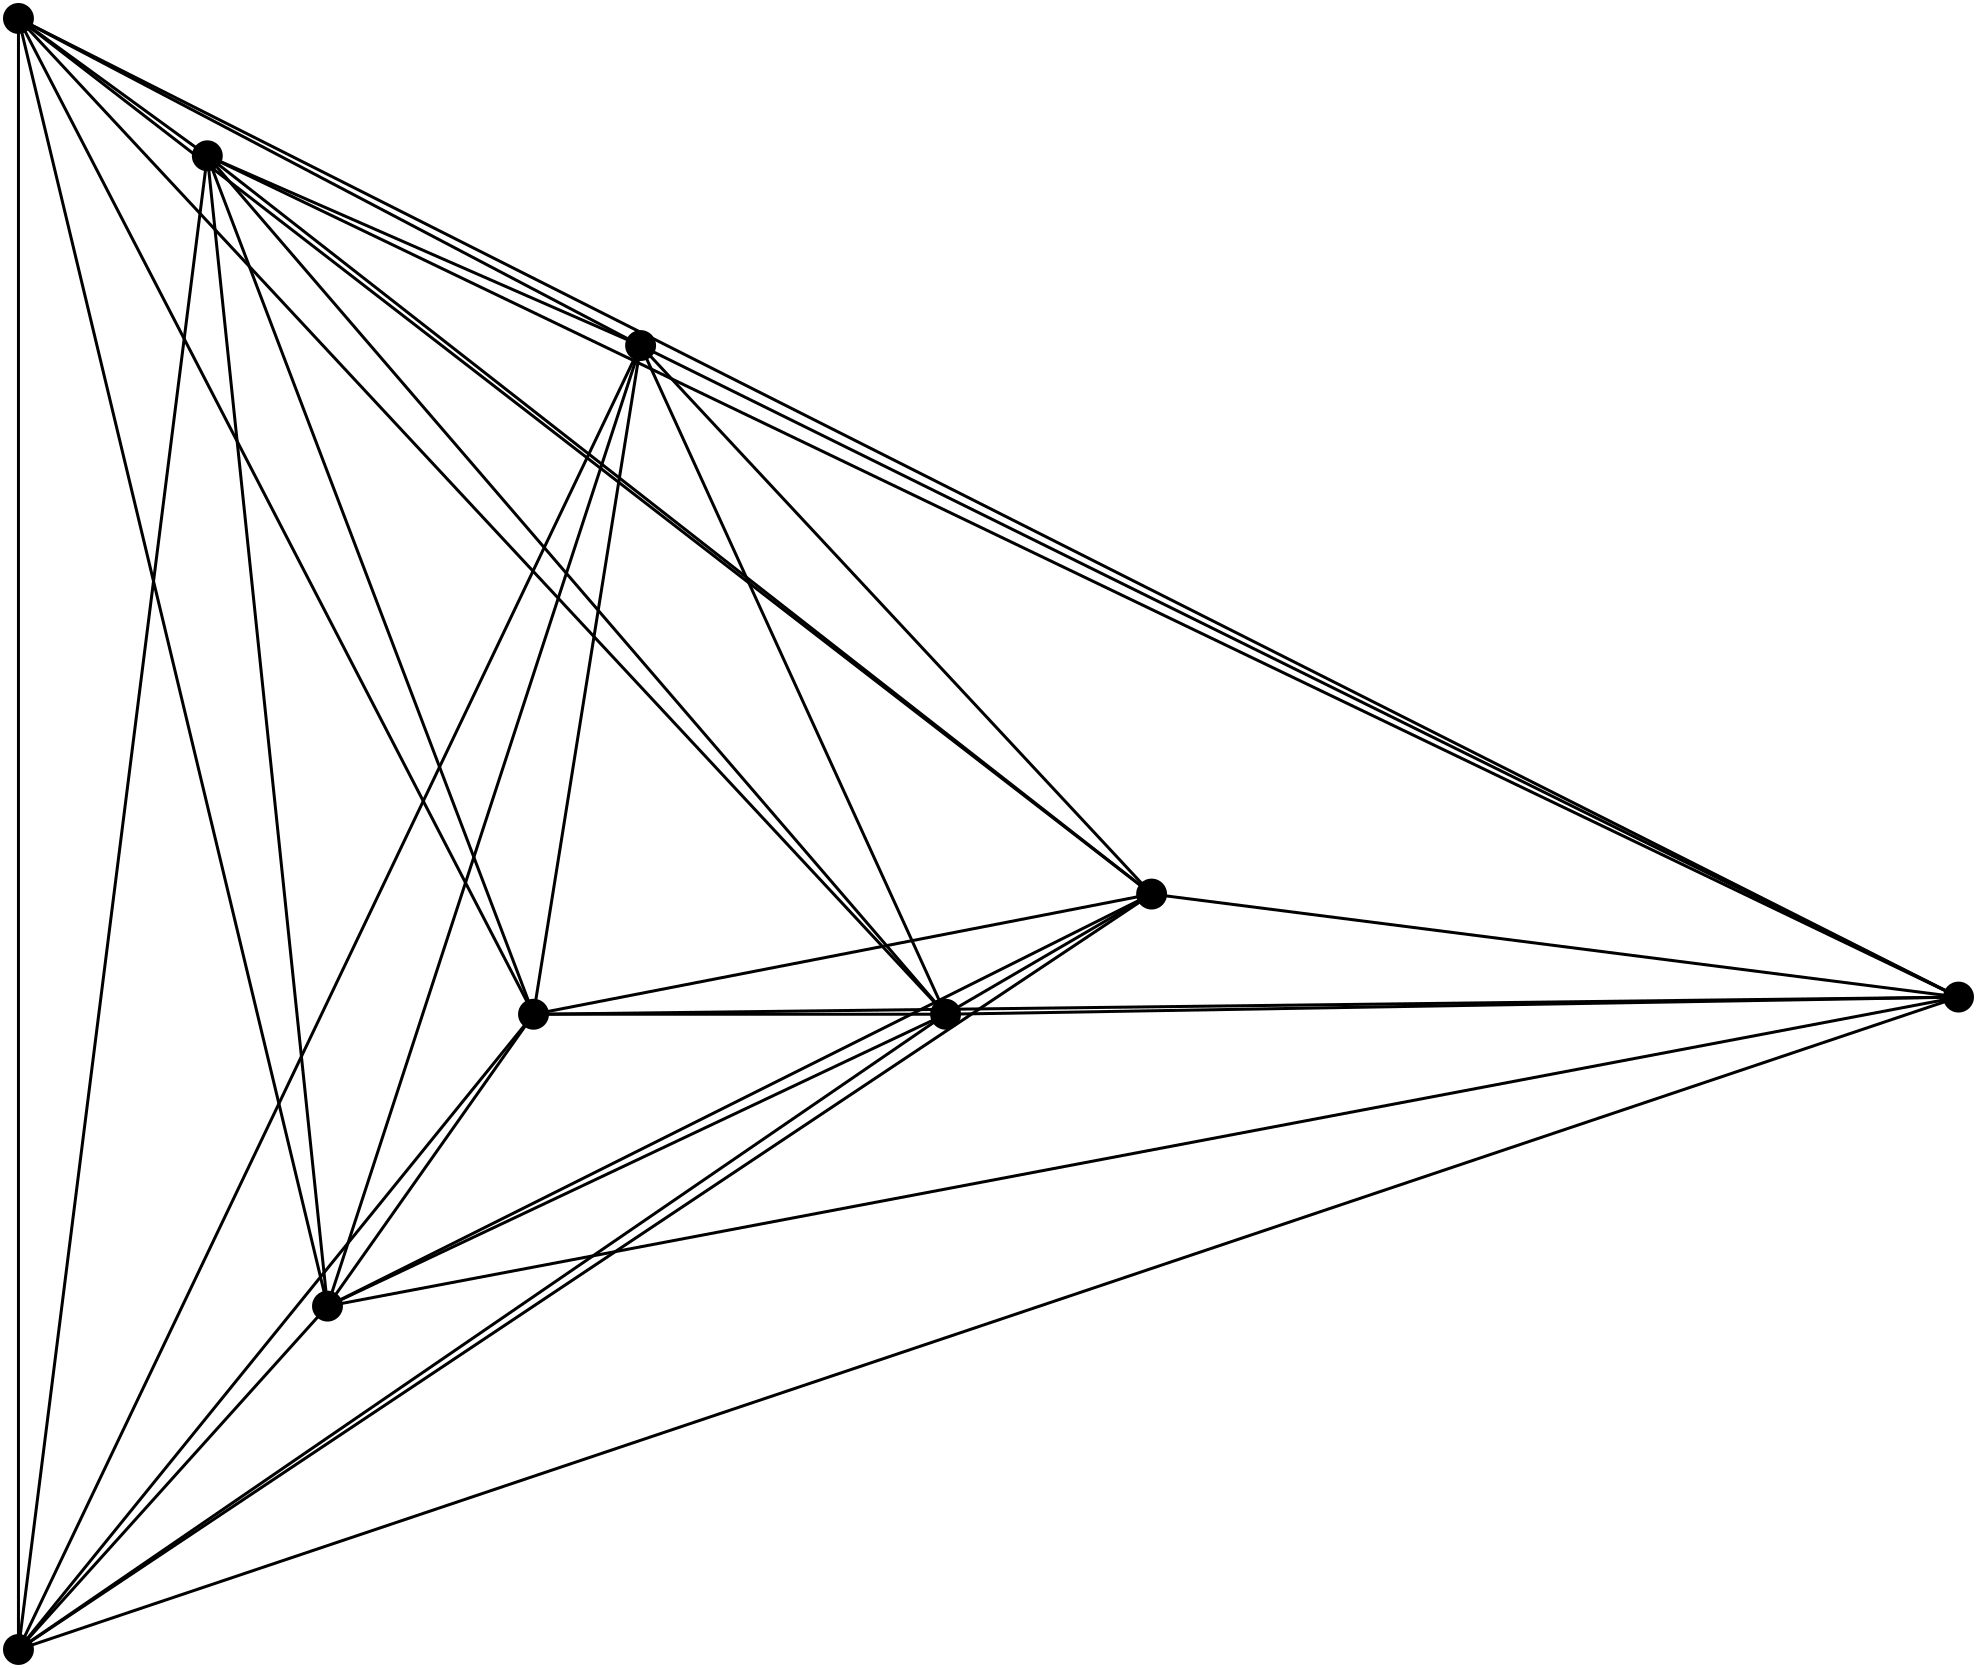
\includegraphics[width=0.8\textwidth]{k9_nomax}
    \caption{Este conjunto de puntos corresponde al tipo de orden 136764 de $n=9$.
    La gráfica completa inducida por ellos no contiene ningún thrackle máximo.}
    \label{k9_nomax}
  \end{figure}
  \begin{table}
    \centering
    \setlength\extrarowheight{2pt}
    \begin{tabularx}{\textwidth}{|C|l|l|l|}
      \hline
      $n$ & Tipos de orden(T.O.) & \makecell{T.O. con solo\\ un thrackle máximo} &
       \makecell{T.O. sin \\thrackles máximos\hfill} \\\hline
      3 & 1         & 1(33\%)         & 0(0\%)    \\
      4 & 2         & 0(0\%)          & 1(50\%)   \\
      5 & 3         & 0(0\%)          & 2(66\%)   \\
      6 & 16        & 1(6.25\%)       & 6(37.50\%)  \\
      7 & 135       & 7(5.18\%)       & 50(37.03\%) \\
      8 & 3315      & 208(6\%)        & 1175(35.44\%) \\
      9 & 158817    & 10547(6.64\%)   & 53758(33.84\%) \\
      10 & 14309547 & 962517(6.72\%)  & 4654339(32.52\%) \\ \hline
    \end{tabularx}
    \caption{Mostramos, para cada $3\leq n \leq 10$,
    la relación de los tipos de orden con solamente un thrackle máximo y
    los tipos de orden sin thrackles máximos.}
    \label{tabla_relacion_ot}
  \end{table}

  Los algoritmos que diseñamos para dar los resultados anteriores son descritos
  en la sección \ref{seccion_algoritmos} para no romper con el flujo de esta
  sección. Para buscar los thrackles máximos usamos el
  algoritmo~\ref{algo_kthrackles}, para comparar los thrackles a pares utilizamos
  el algoritmo~\ref{algo_interseccion}. La lista de tipos de orden
  con un solo thrackle máximo puede ser descargada de la siguiente liga:
  \url{http://computacion.cs.cinvestav.mx/~dmerinos/site/archivos_tesis/withone_max.tar.gz}.
  La lista de tipos de orden para los cuales no existe un thrackle máximo
  está en la siguiente liga:
  \url{http://computacion.cs.cinvestav.mx/~dmerinos/site/archivos_tesis/without_max.tar.gz}.

  Usando estos resultados podemos derivar el siguiente lema.
  \begin{lemma}\label{lema:thdisjuntos}
    Sea $S$ un conjunto de puntos en posición general y sean $T_1$ y $T_2$ thrackles máximos en $K_n(S)$
    con $|V(T_1)|\leq 10$ y $|V(T_2)|\leq 10$. $T_1$ y $T_2$ tienen al menos una arista en común.
  \end{lemma}
  \begin{proof}
    Esta demostración se obtuvo computacionalmente. Para cada tipo de orden con hasta diez puntos,
    generamos todos los thrackles  máximos inducidos con el algoritmo~\ref{algo_kthrackles} cuya
    correctitud discutimos en la sección~\ref{seccion_algoritmo_kthrackles}. Usando este conjunto
    verificamos que para cada pareja la intersección en aristas es no vacía usando el
    algoritmo~\ref{algo_interseccion} que describimos en la
    sección~\ref{secc:algo_interseccion_thrackles}.
  \end{proof}

  El lema anterior implica que para $n\leq 10$ no es posible encontrar una
  descomposición en thrackles máximos de tamaño
  $\left\lceil\frac{n-1}{2}\right\rceil$, ya que, si esta exisitiera, los
  thrackles máximos no serían disjuntos a pares y esto infringiría las
  condiciones de una descomposición.
  En otras palabras una descomposición por thrackles solo podría contener un
  thrackle máximo. Sin embargo, es posible encontrar, a partir de una colección
  de thrackles máximos, una colección de thrackles que son disjuntos (y no necesariamente máximos).
  Describimos este proceso en el siguiente lema:
  % Por consecuencia es posible contar cuántas aristas son cubiertas
  % por una descomposición de thrackles máximos cuyo tamaño es $\left\lceil\frac{n-1}{2}\right\rceil$.
  \begin{lemma}\label{lema:existedescomp}
    Sea $\mathcal{C}=\{T_1,T_2,\dots,T_m\}$ una colección de thrackles máximos
    de $K_n$ con $|E(T_i)\cap E(T_j)| = 1$ y $ i,j \in \{1,2,\dots,m\}$.
    Existe una colección  de thrackles $\mathcal{D}$ de $K_n$ inducida por
    $\mathcal{C}$ en la que cada par de thrackles tienen intersección vacía y que
    cubre el siguiente número de aristas:
    \[\displaystyle \sum^n_{i=(n-m) + 1}i.\]
  \end{lemma}
  \begin{proof}
    Sea $T'_i$, con $1 \leq i \leq m$ un thrackle inducido por el siguiente
    conjunto de aristas:
    \[E(T_i) - \bigcup_{k=1}^{i-1} E(T_i)\cap E(T_k).\]

    Es decir, $T'_i$ es el thrackle que tiene todas las aristas de $T_i$
    a excepción de aquellas que $T_i$ comparte con el resto de los thrackles
    en la colección.

    Sea $\mathcal{D}=\{T'_1,T'_2,\dots,T'_m\}$. Por construcción, la intersección
    de cualesquiera dos thrackles de $\mathcal{D}$ es vacía.

    Nótese que si una arista $e$ aparece en dos thrackles de $\mathcal{C}$,
    entonces en $\mathcal{D}$, $e$ aparecerá únicamente en el thrackle con menor
    etiqueta.
    De hecho $T_1'$ tiene $n$ aristas, $T_2'$ tiene $n-1$ aristas, $T_3'$ tiene
    $n-2$ aristas y, en general, $T_i'$ tiene $n-i+1$ aristas. Como $\mathcal{D}$
    tiene $m$ thrackles el número de aristas cubiertas por $\mathcal{D}$ es
    \[ n + (n-1) + (n-2) + \cdots + (n- m + 2) + (n - m + 1).\]
    Podemos escribir esta suma como :
    \[\displaystyle \sum^n_{i=(n-m) + 1}i.\]
  \end{proof}
  Es importante notar que este es el máximo número de aristas que una colección
  con $m$ thrackles disjuntos puede cubrir.
  % Es importante notar que este es el número más grande de aristas cubiertas por
  % una colección de thrackles disjuntos en aristas inducida por una colección de
  % thrackles máximos, esto es debido a que en el lema~\ref{lema:thdisjuntos}
  % consideramos que la intersección en aristas de dos thrackles máximos es de
  % tamaño 1. No es difícil observar que si la intersección es más grande entonces
  % el número de aristas cubiertas por la colección inducida es menor.

  Con los lemas anteriores es posible probar que la cota inferior del
  anti-thickness geométrico de $K_n$, mostrada en la ecuación
  \ref{ecuacion_cotas_atg}, no es justa para toda $n$. El siguiente teorema
  establece esta afirmación.
  \begin{theorem}\label{teo:cotainf}
  Sea $\mathcal{D}=\{T'_1,T'_2,\dots,T'_{\left\lceil\frac{n-1}{2}\right\rceil}\}$
  una colección de thrackles disjuntos en aristas inducida por una colección de
  $\left\lceil\frac{n-1}{2}\right\rceil$ thrackles máximos.
  $\left\lceil\frac{n-1}{2}\right\rceil$ thrackles máximos son
  suficientes para inducir una descomposición de $K_n$ cuando $n\in \{3,4,6\}$ y no son suficientes cuando $n\in\{5,7,8,9,10\}$.
  \end{theorem}
  \begin{proof}
    Se sigue del lema~\ref{lema:existedescomp}. El número de aristas cubiertas
    por $\mathcal{D}$ para cada $3\leq n \leq 10$ se muestran en la
    tabla~\ref{table:attrivialtight}. Observando la tercera columna, es claro que para
    $n\in\{5,7,8,9,10\}$, $\left\lceil\frac{n-1}{2}\right\rceil$ thrackles máximos no cubren las aristas
    necesarias de la gráfica completa. Marcamos estos casos de gris.
  \end{proof}
  % En la tabla~ mostramos los casos para los que la cota
  % inferior del anti-thickness geométrico no es justa usando el
  % lema~\ref{lema:existedescomp}.
  % Es importante notar que este resultado es válido solamente cuando el dibujo de
  % $K_n$ tiene al menos
  % $\left\lceil\frac{n-1}{2}\right\rceil$ thrackles máximos.

  \begin{table}[t]
    \centering
    \begin{tabular}{|c|c|c|c|}
      \hline
      $n$ & $\left\lceil\frac{n-1}{2}\right\rceil$ &
      $\sum^n_{i=\left(n-\left\lceil\frac{n-1}{2}\right\rceil\right) + 1}i$ &
      $\binom{n}{2}$\\[5pt] \hline\hline
      3   & 1  & 3 & 3 \\ \hline
      4   & 2  & 7 & 6 \\ \hline
      5   & 2  & \cellcolor{red!25}9 & 10 \\ \hline
      6   & 3  & 15 & 15 \\ \hline
      7   & 3  & \cellcolor{red!25}18 & 21 \\ \hline
      8   & 4  & \cellcolor{red!25}26 & 28 \\ \hline
      9   & 4  & \cellcolor{red!25}30 & 36 \\ \hline
      10  & 5  & \cellcolor{red!25}40 & 45 \\ \hline
    \end{tabular}
    \caption{ Mostramos cuántas aristas son cubiertas con una colección de
    $\left\lceil\frac{n-1}{2}\right\rceil$ thrackles máximos disjuntos en
    aristas. Se rellenan los casos en los que la colección no cubre todas las
    aristas. }
    \label{table:attrivialtight}
  \end{table}

  Como consecuencia del lema~\ref{lema:existedescomp} y el teorema~\ref{teo:cotainf} podemos dar una cota inferior justa para el anti-thickness geométrico de $K_n$ con $3 \leq n \leq 10$.

  \begin{theorem}\label{teo:nuevacotainf}
    Sea $S$ un conjunto de $n$ puntos en el plano en posición general con $3\leq n \leq 10$, y sea $K_n(S)$ la gráfica completa inducida por $S$. El anti-thickness $At_g(K_n)$ de $K_n(S)$ tiene la siguiente cota inferior:
    \begin{equation}
      At_g(K_n) \geq n - \left\lfloor\sqrt{2n+\frac{1}{4}} - \frac{1}{2}\right\rfloor.
      \label{ecuacion_cota_inf}
    \end{equation}
  \end{theorem}
  \begin{proof}
    Se sigue del teorema ~\ref{lema:existedescomp} que el número de aristas
    cubiertas por una colección $\mathcal{D}=\{T_1,T_2,\dots,T_m\}$ de thrackles,
    con $|E(T_i)\cap E(T_j)| = 1$, es
    \[ -\frac{1}{2}m(m-2n-1). \]
    Para saber cuántos thrackles como mínimo son necesarios en la colección para
    cubrir las $\binom{n}{2}$ aristas de $K_n$, es necesario resolver la
    siguiente desigualdad otorga el resultado.
    \begin{equation}
       -\frac{1}{2}m(m-2n-1) \geq \binom{n}{2}.
       \label{ecuacion_desigualdad_cota_inf}
    \end{equation}

    De aquí se tiene que $m$ está en el siguiente intervalo:
    \[
      \frac{1}{2}\left(2n-\sqrt{8n+1} + 1\right) \leq m \leq  \frac{1}{2}\left(2n+\sqrt{8n+1} + 1\right).
    \]
    Como nosotros estamos interesados en la $m$ más pequeña para la cual se cumple la desigualdad~\ref{ecuacion_desigualdad_cota_inf}, basta con tomar el término de la izquierda para obtener el resultado deseado.
  \end{proof}
    Presentamos los valores dados por la cota inferior del
    teorema~\ref{teo:nuevacotainf} en la tabla~\ref{table:atnuevacota}.
    Es posible observar que para toda $n$, con $3\leq n\leq 10$ se cubren las aristas de la gráfica completa si usamos $n - \left\lfloor\sqrt{2n+\frac{1}{4}} - \frac{1}{2}\right\rfloor$ thrackles máximos
    en la colección.
    \begin{table}[t]
      \centering
      \begin{tabular}{|c|c|c|c|}
        \hline
        $n$ & $k=n - \left\lfloor\sqrt{2n+\frac{1}{4}} - \frac{1}{2}\right\rfloor$ & $\sum^n_{i=(n-k) + 1}i$ & $\binom{n}{2}$\\[5pt] \hline\hline
        3   & 1  & 3 & 3 \\ \hline
        4   & 2  & 7 & 6 \\ \hline
        5   & 3  & 12 & 10 \\ \hline
        6   & 3  & 15 & 15 \\ \hline
        7   & 4  & 22 & 21 \\ \hline
        8   & 5  & 30 & 28 \\ \hline
        9   & 6  & 39 & 36 \\ \hline
        10  & 6  & 45 & 45 \\ \hline
      \end{tabular}
      \caption{En la tabla se muestra que la cota inferior del anti-thickness
      geométrico es justa para $3 \leq n \leq 10$. La segunda columna muestra el
      tamaño de la colección de thrackles, cuyo tamaño está dado por la cota
      inferior del anti-thickness geométrico del teorema~\ref{teo:nuevacotainf}
      para cada $n$. La tercera columna muestra cuántas aristas cubre dicha
      colección. La cuarta columna muestra el número de aristas de $K_n$.}
      \label{table:atnuevacota}
    \end{table}

    Como consecuencia del teorema~\ref{teo:nuevacotainf} es posible obtener un valor exacto para el anti-thickness geométrico de $K_n$ en posición general.
    \begin{theorem}\label{teo:cotaexacta}
      Sea $K_n(S)$ la gráfica completa inducida por un conjunto $S$ de $n$ puntos, con $3 \leq n \leq 10$, en posición general. El anti-thickness geométrico de $K_n$ es:
      \[ At_g(K_n) = n - \left\lfloor\sqrt{2n + \frac{1}{4}} - \frac{1}{2}\right\rfloor. \]
    \end{theorem}
    \begin{proof}
      Se sigue del resultado del teorema~\ref{teo:nuevacotainf} y
      la cota superior~(\cite{Fabila-Monroy2018}) del anti-thickness geométrico de $K_n$,
      $n - \left\lfloor\sqrt{2n + \frac{1}{4}} - \frac{1}{2}\right\rfloor $ , cuando
      $K_n$ es inducida por un conjunto de puntos en posición convexa.
    \end{proof}

    Para dar un resultado similar para $n > 10$, bastaría con generalizar el
    lema~\ref{lema:thdisjuntos}. Esto es, demostrar que cada par de thrackles máximos se
    intersecta en al menos una arista y que esto sucede para toda $n > 10$. Nosotros
    conjeturamos que este lema también se cumple para $n>10$.

    Debido a que la cota superior del anti-thickness geométrico está dada por
    el dibujo en posición convexa, en este trabajo decidimos verificar si existen
    dibujos diferentes al convexo, para los cuales se alcanza la cota inferior
    dada por el teorema~\ref{teo:nuevacotainf}. Hacemos esto en la siguiente sección.

\section{Cota superior del anti-thickness geométrico}\label{secc:descomposicion_thrackles_maximos}

  La cota superior del anti-thickness geométrico está dada por el conjunto
  de puntos en posición convexa. Sea $k=n - \left\lfloor\sqrt{2n+\frac{1}{4}} -
  \frac{1}{2}\right\rfloor$, en esta tesis verificamos que existen tipos de
  orden, que no corresponden a la posición convexa, y que inducen una gráfica
  completa cuyo anti-thickness geométrico es a lo sumo $k$.

  Para comprobar la existencia de tipos de orden con las características descritas
  anteriormente elegimos aquellos que tienen al menos $k$ thrackles
  máximos. Luego, para cada uno, analizamos todas sus colecciones de thrackles
  máximos de tamaño $k$. Finalmente, para cada colección, evaluamos si
  esta cubre o no a $E(K_n)$. Cuando una colección de thrackles máximos cubre
  al conjunto de aristas de la gráfica completa, es posible inducir una descomposición
  de $K_n$ en thrackles (no necesariamente máximos) asignando cada arista de $K_n$
  a un único thrackle que la cubra. Detallamos el algoritmo para buscar
  colecciones de thrackles máximos que induzcan una descomposición en la sección
  \ref{secc:algo_descomposicion_thrackles_maximos}. La tabla~\ref{table:res_desc_th_max}
  muestra los resultados que obtuvimos de este análisis; observamos que únicamente para
  $n\in \{8,9,10\}$ existen tipos de orden que tienen $k$ thrackles máximos que
  pueden inducir una descomposición.

  Con los resultados del algoritmo~\ref{algo_kthrackles} de búsqueda de thrackles podemos decir que
  las gráficas completas inducidas por los tipos de orden de la tabla~\ref{table:res_desc_th_max}
  no son necesariamente las que tienen más thrackles máximos. Mostramos cuántos thrackles máximos
  hay en cada tipo de orden en un archivo que puede ser descargado de la liga~\ref{link-thrMax_k}
  del apéndice~\ref{apendice-ligas}. Para $n\in\{8,9,19\}$ el tipo de orden con más thrackles
  máximos es el de etiqueta 1 o en otras palabras el siguiente del tipo de orden en posición
  convexa. Para estos tipos de orden existen 94, 213 y 459 thrackles máximos respectivamente.

  El porcentaje de tipos de orden de $8,9$ y $10$ puntos para los cuales es posible inducir una
  descomposición usando solamente thrackles máximos son los siguientes: solo el $0.09\%$ de los
  tipos de orden de 8 puntos tiene una descomposición en thrackles máximos incluyendo la posición
  convexa, solo el $0.005\%$ de los tipos de orden de 9 puntos y solo el $.00002\%$ de los tipos de
  orden de 10 puntos.

  Si la intersección de cada par de thrackles de la colección es exactamente de tamaño 1, entonces
  la colección es óptima, de otra manera, la colección no es óptima. Verificamos la optimalidad de
  las colecciones de thrackles máximos y encontramos  que ninguna colección, para los tipos de
  orden descritos anteriormente, es óptima ya que en cada una existe al menos un par de thrackles
  cuya intersección tiene tamaño mayor a uno. Para este proceso utilizamos el
  algoritmo~\ref{algo_interseccion} de intersección de thrackles descrito en la
  sección~\ref{secc:algo_interseccion_thrackles}. Este resultado nos permite dar el siguiente
  teorema.

  \begin{theorem}\label{teo:coleccion_optima}
    Sea $K_n(S)$ una gráfica completa inducida por un conjunto $S$ de $n$ puntos,
    con $3\leq n\leq 10$ , en posición general no convexa. No existen
    colecciones de thrackles máximos óptimas en $K_n(S)$.
  \end{theorem}
  \begin{proof}
    Esta demostración se obtuvo computacionalmente. Se sigue del algoritmo de búsqueda de
    colecciones de thrackles máximos que induzcan una descomposición cuya correctitud es discutida
    en la sección~\ref{secc:algo_descomposicion_thrackles_maximos} y de la verificación de
    optimalidad. Encontramos que no existe ninguna colección de thrackles máximos óptima para
    ningún tipo de orden diferente del convexo para $3\leq n\leq 10$.
  \end{proof}

  % Es importante hacer notar que encontramos configuraciones de puntos,
  % en posición no convexa, cuyo anti-thickness geométrico es $n -
  % \left\lfloor\sqrt{2n+\frac{1}{4}} - \frac{1}{2}\right\rfloor$.
  Las etiquetas de los thrackles máximos para las gráficas dadas por cada tipo de orden de los
  mostrados en la tabla~\ref{table:res_desc_th_max} pueden ser consultados en el
  apéndice~\ref{apendice_thrackles_inducen}.

  La figura~\ref{fig:k9_descomp} muestra un ejemplo de una descomposición de $K_9$ en thrackles,
  inducida por seis thrackles máximos, cada thrackle es dibujado de un color diferente.

  \begin{figure}
    \centering
    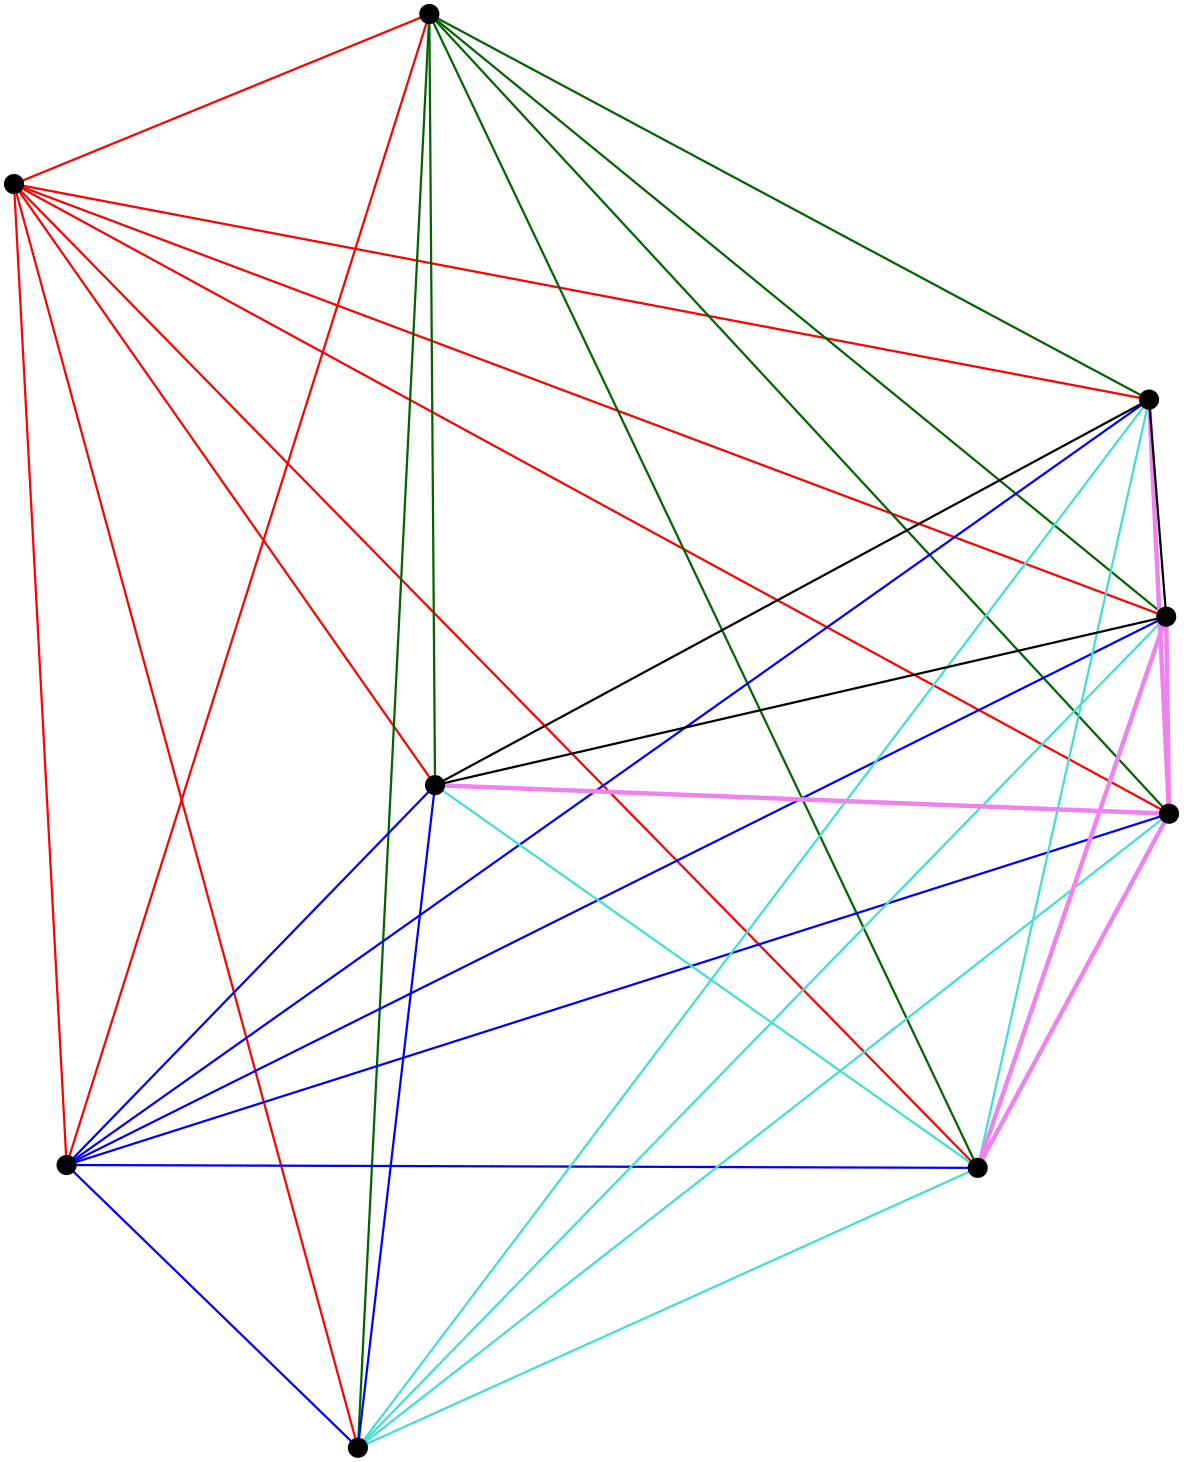
\includegraphics[width=0.7\textwidth]{k9_descomp_2}
    \caption{Una descomposición de $K_9$ en seis thrackles, la configuración de
    puntos corresponde al tipo de orden 12 con respecto de la base de datos
    de~\cite{Aichholzer2001}. El anti-thickness geométrico de $K_9$ es
    6. Esta descomposición fue inducida por una colección
    de thrackles máximos que no es óptima, es sencillo ver esto observando que
    los thrackles tienen 9,7,6,6,5 y 3 aristas respectivamente.
    Una descomposición óptima de $K_9$ tiene thrackles de tamaño 9,8,7,6,5 y 4.}
    \label{fig:k9_descomp}
  \end{figure}

  \begin{table}[]
    \centering
    \setlength\extrarowheight{2pt}
    \begin{tabularx}{\textwidth}{|C|C|C|C|}
      \hline
      $n$   & Tipo de Orden & Tamaño de la colección \hfill $n -
      \left\lfloor\sqrt{2n+\frac{1}{4}} - \frac{1}{2}\right\rfloor$ & No. thrackles máximos \\ \hline\hline
      8 & 12   & 5 & 38  \\
      8 & 54   & 5 & 33  \\ \hline
      9 & 12   & 6 & 103 \\
      9 & 52   & 6 & 101 \\
      9 & 54   & 6 & 83  \\
      9 & 80   & 6 & 75  \\
      9 & 696  & 6 & 80  \\
      9 & 1080 & 6 & 40  \\
      9 & 1287 & 6 & 64  \\ \hline
     10 & 81   & 6 & 177 \\
     10 & 1328 & 6 & 151 \\
     10 & 2243 & 6 & 129  \\ \hline
    \end{tabularx}
    \caption{Tipos de orden para los que existe al menos una colección de
    $n -
    \left\lfloor\sqrt{2n+\frac{1}{4}} - \frac{1}{2}\right\rfloor$ thrackles máximos que cubren a
    $K_n$.}
    \label{table:res_desc_th_max}
  \end{table}

  Decidimos estudiar la estructura geométrica de los tipos de orden de la
  tabla~\ref{table:res_desc_th_max} para intentar caracterizar cuáles conjuntos de puntos inducen
  una gráfica completa que tiene una descomposición en thrackles máximos. Para esto describimos a
  continuación el concepto de \emph{k-convexidad}(~\cite{Valtr2002}) de un conjunto y
  \emph{reflexividad} de un conjunto.
  Existen varias definiciones de un conjunto $k$-convexo, aquí retomamos una.
  \newpage

  \begin{definition}{(\cite{Valtr2002})\emph{Conjunto k-convexo}.}
    Un conjunto $P$ de puntos en el plano es $k$-convexo si ningún triángulo definido por tres
    puntos de $P$ contiene a más de $k$ puntos de $P$ en su interior.
  \end{definition}
  Un conjunto de puntos en posición convexa es claramente 0-convexo ya que cualquier triángulo
  definido por tres puntos dicho conjunto, no contiene a ningún otro punto del conjunto. En la
  figura~\ref{fig:2convex} mostramos un conjunto que es 2-convexo.

  \begin{figure}
    \centering
    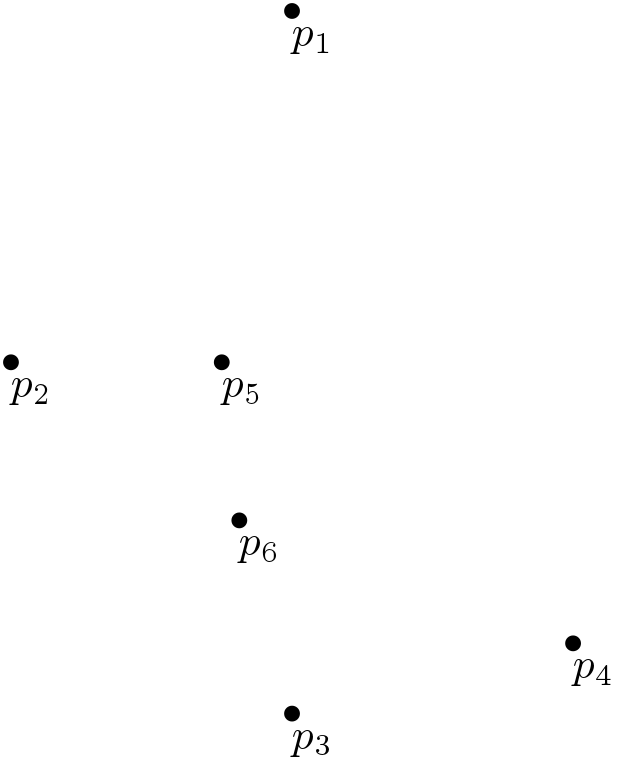
\includegraphics[width=0.4\linewidth]{2convex}
    \caption{Un conjunto de puntos 2-convexo según la definición de \cite{Valtr2002}, nótese que
    los puntos $p_1$,$p_2$ y $p_3$ inducen un triángulo con dos puntos en su interior y que ningún
    otro triángulo inducido por el conjunto tiene a más de dos puntos en su interior.}
    \label{fig:2convex}
  \end{figure}

  Para la siguiente definición consideramos una \emph{poligonización} de un conjunto $Q$ de
  puntos como un polígono cuyo conjunto de vértices es $Q$.

  \begin{definition}{(\cite{Arkin2003})\emph{Reflexividad de un conjunto}.}
    Sea $r(P)$ el número de vértices cóncavos de un polígono $P$ y sea $\mathcal{P}$ el conjunto de
    todas las poligonizaciones de un conjunto $S$ de puntos, la reflexividad del conjunto $S$ se
    define como sigue: \[ \rho(S) = \min_{P\in \mathcal{P}} r(P).\]
  \end{definition}

  Es sencillo notar que cualquier conjunto en posición convexa tiene reflexividad 0, ya que todos
  sus ángulos son convexos.

  Basándonos en las definiciones anteriores encontramos que, de los tipos de orden en la
  tabla~\ref{table:res_desc_th_max}, los doce tienen reflexividad igual a uno. Esto es, que todos
  tienen una poligonización que cuenta con solamente un vértice cóncavo. Cuando un conjunto de $n$
  vértices tiene a $n-1$ vértices en posición convexa y a un vértice dentro de la cubierta convexa,
  es fácil observar que la reflexividad es uno, puesto que la cadena convexa contiene a $n-1$
  vértices y solo es necesario unir, con dos aristas, el principio y el fin de dicha cadena con el
  vértice que está dentro de la cadena convexa. El tipo de orden número 1080 para $n=9$ contiene a
  dos puntos en el interior de su cubierta convexa, sin embargo, es posible encontrar una
  poligonización con un solo ángulo cóncavo. Presentamos dicha poligonización en la
  figura~\ref{fig:poligonizacion1080}.

  Respecto a la $k$-convexidad, encontramos que todos los tipos de orden listados, a excepción del
  tipo de orden de nueve vértices con número 1080, son $1$-convexos ya que cuentan con solamente un
  punto en el interior de su cubierta convexa; el tipo de orden con número 1080 es $2$-convexo.

  Es importante recalcar que estos conjuntos son similares a la posición convexa, recordemos que la
  posición convexa tiene reflexividad 0 y todos los tipos de orden para los que existe una
  descomposición en thrackles inducida por thrackles máximos tienen reflexividad 1, en este
  sentido, la reflexividad de los conjuntos no es distante. Por otra parte, los conjuntos en
  posición convexa son $0$-convexos mientras que la mayoría de los tipos de orden anteriormente
  descritos son 1-convexos, a excepción de un conjunto que es 2-convexo, de nuevo estos valores no
  distan mucho de la convexidad del conjunto en posición convexa.

  \begin{figure}
    \centering
    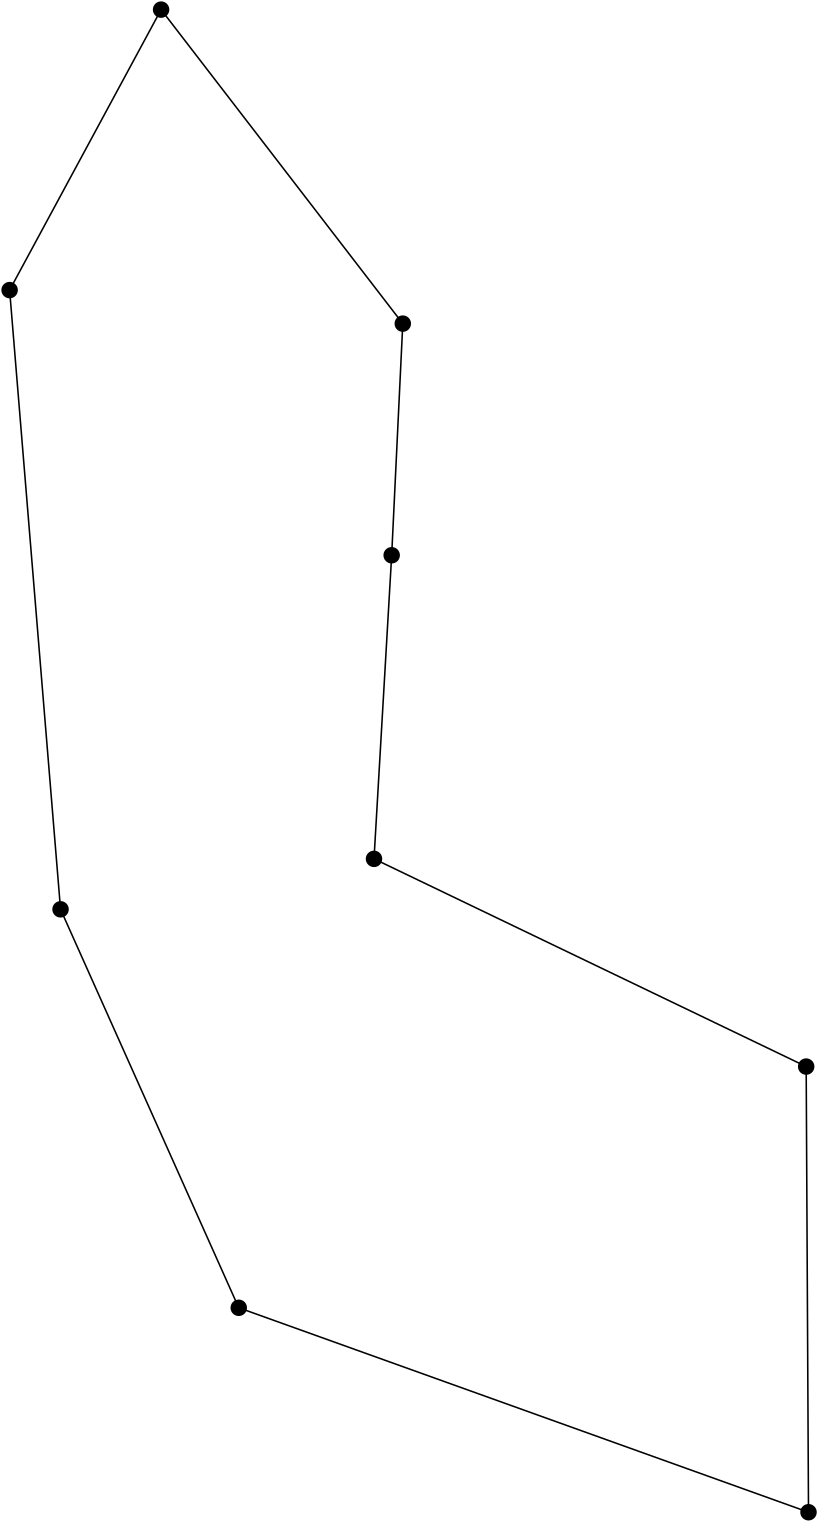
\includegraphics[width=0.5\textwidth ]{poligonizacion1080}
    \caption{Una poligonización para el tipo de orden número 1080 de nueve vértices, esta poligonización solo tiene un ángulo cóncavo por lo que su reflexividad es uno. No es cero ya que esto requiere que todos sus ángulos sean convexos, lo que equivale a que todos los puntos estén en posición convexa.}
    \label{fig:poligonizacion1080}
  \end{figure}

  Para los casos de $n \in \{3,4,\dots,7\}$ no existe ninguna
  colección de $k$ thrackles máximos que pueda inducir una descomposición de
  $K_n$. Esto es porque, para ninguno de los tipos de orden, en este rango de $n$,
  existe una colección de thrackles máximos que cubran las aristas de $K_n$ (a excepción del
  dibujo en posición convexa). Creemos que una de las razones por las que esto sucede es que los
  thrackles máximos que existen para cada tipo de orden en este rango comparten muchas aristas a
  pares por lo que aunque exista un alto número de thrackles máximos, la unión no cubre las aristas
  de la gráfica completa.

  Para los valores de $n$ anteriormente mencionados buscamos, de manera manual, una descomposición
  con ese número de thrackles (no necesariamente máximos). Explicamos esto en la
  sección~\ref{secc:interseccion_thrackles}.

  La figura~\ref{fig:descomposicionesk4_k9} muestra para cada valor de $n$ con $3\leq n\leq 7$,
  dibujos cuyo anti-thickness  es igual a la cota inferior del teorema~\ref{teo:nuevacotainf}. De
  esto se sigue que el anti-thickness geométrico de $K_n$, con $ 3 \leq n \leq 7$, es a lo
  sumo $n - \left\lfloor\sqrt{2n+\frac{1}{4}} - \frac{1}{2}\right\rfloor$.
  Como resultado podemos decir que el anti-thickness geométrico de $K_n$, con $ 3\leq n \leq 10$
  es exactamente $n - \left\lfloor\sqrt{2n+\frac{1}{4}} - \frac{1}{2}\right\rfloor$.

  \begin{figure}[htpb]
    \centering
    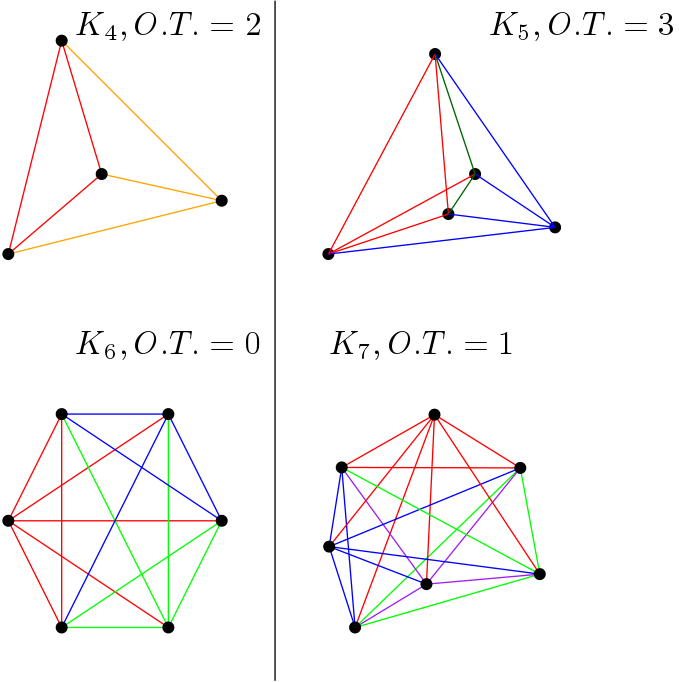
\includegraphics[width=0.7\textwidth]{descomposiciones_K49.png}
    \caption{Mostramos posibles descomposiciones de la gráfica completa con
    hasta 7 vértices. Las descomposiciones tienen exactamente el número de
    thrackles establecido por la cota inferior del
    teorema~\ref{teo:nuevacotainf}. Estas configuraciones de puntos, a excepción de $K_6$, son
    diferentes de la posición convexa. Los tipos de orden correspondientes a cada dibujo están
    indicados en la figura como $O.T.$}
    \label{fig:descomposicionesk4_k9}
  \end{figure}

  Mientras estudiábamos las colecciones de thrackles máximos, decidimos explorar en qué otra forma
  se parecen los tipos de orden de la tabla~\ref{table:res_desc_th_max} a la posición convexa y por
  ello buscamos calcular el número de cruce de los thrackles máximos de las colecciones, detallamos
  los resultados de este análisis en la siguiente sección.

  \subsection{Número de cruce de thrackles máximos }\label{secc:cnthracklemax}

    Durante el desarrollo de este trabajo decidimos analizar el número de cruce
    de cada uno de los thrackles máximos que hay en una colección que puede inducir una
    descomposición de $K_n$. Definimos el número de cruce de una gráfica geométrica a continuación.

    \begin{definition}{\emph{Número de cruce de una gráfica geométrica}(\cite{Schaefer2018})}
      El número de cruce $cr(\mathsf{G})$ de una gráfica geométrica $\mathsf{G}$
      es el número de cruces propios entre aristas de $\mathsf{G}$.
    \end{definition}

    Mostramos ejemplos del número de cruce de gráficas geométricas en la
    figura~\ref{fig:k4_cn}; es posible observar que la gráfica $K_4$ puede ser dibujada con
    un cruce y también puede ser dibujada como gráfica plana (sin cruces).
    \begin{figure}[h]
      \centering
      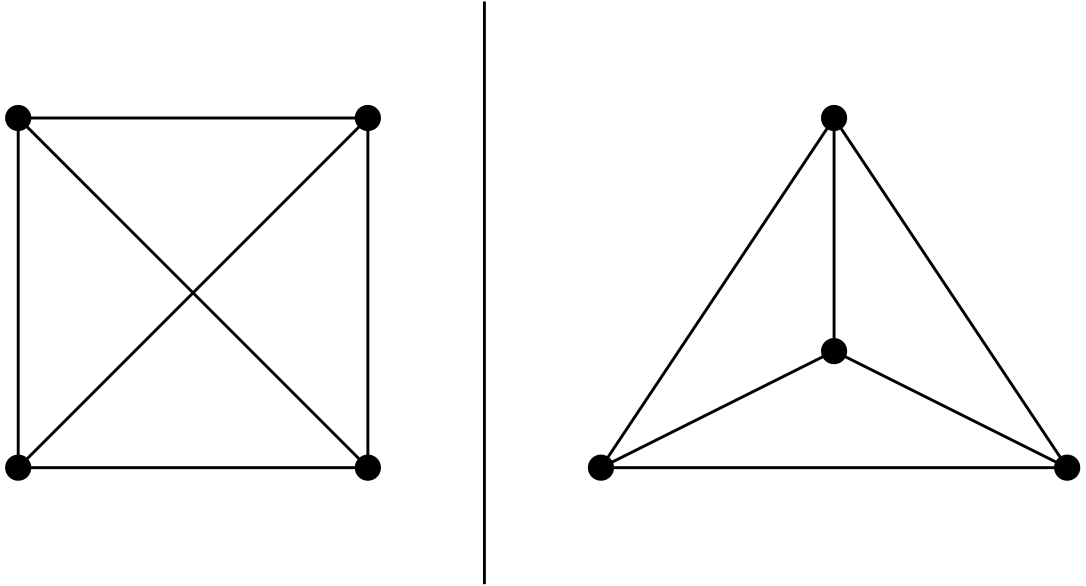
\includegraphics[width=0.5\textwidth]{k4_cn}
      \caption{A la izquierda, $K_4$ dibujada con un cruce. A la derecha $K_4$ dibujada sin
      cruces.}
      \label{fig:k4_cn}
    \end{figure}

    Para presentar los resultados de esta sección, debemos definir el número de cruce de un thrackle
    máximo. Para esto, es necesario mencionar cuántos \emph{no cruces} existen en un thrackle
    geométrico. Para nosotros, un \emph{no cruce} es un par de aristas que son adyacentes
    entre sí.

    \begin{lemma} \label{lema:nocruces}
      Sea $T$ un thrackle y sea $v\in V(T)$ un vértice de $T$. El vértice $v$ causa
      $\binom{deg(v)}{2}$ \emph{no cruces}. En otras palabras: existen $\binom{deg(v)}{2}$ aristas
      adyacentes a pares para cada vértice $v\in V(T)$.
    \end{lemma}
    \begin{proof}
      Sea $e=(a,b)$ una arista de $T$ con extremos $a$ y $b$. Por la definición de thrackle
      geométrico toda arista diferente de $e$, con extremo en $a$ o en $b$ es adyacente con
      $e$, y por lo tanto no la cruza. Sea $v\in V(T)$ un vértice con grado $deg(v)=k$ y sea
      $(v,b_i)$ alguna arista con un extremo en $v$, con $1 \leq i \leq k$. Tenemos que $(v,b_i)$
      no cruza a $\{(v,b_{i+1}),(v,b_{i+2})\dots,(v,b_k)\}$, esto es $k-i$ no cruces.
      De esta manera, en total, del vértice $v$ podemos contar $(k-1)+(k-2)+\dots+0$ no cruces, lo
      que equivale a $\binom{k}{2}$ y como, $k=deg(v)$ el resultado se sigue.
    \end{proof}

    \begin{theorem} \label{teorema:cn_thrackle}
      Sea $T$ un thrackle geométrico, con $m=|E({T})|$ el número de cruce $cr({T})$ de ${T}$ es:
      \[
        \binom{m}{2} - \sum_{u \in V({T})} \binom{deg(u)}{2}
      \]
    \end{theorem}
    \begin{proof}
      Como $T$ es un thrackle, cada una de las $m$ aristas debe intersectarse a pares
      exactamente una vez. Si ${T}$ está compuesto solamente por aristas que se cruzan a pares,
      se tiene que para cada $u\in V({T})$ $deg(u)=1$ y por lo tanto $\sum_{u \in V({T})}
      \binom{deg(u)}{2} = 0$ y el resultado se sigue. Sin embargo, debemos tener en cuenta
      que no necesariamente cada par de aristas se cruza sino que algunas pueden ser
      adyacentes. Dicho de otra manera, debemos contar cuántos no cruces existen en el
      thrackle. Por el lema~\ref{lema:nocruces} sabemos que existen exactamente
      $\binom{deg(v)}{2}$ no cruces por cada vértice $v$ del thrackle. El resultado se sigue.
      % Sin embargo, por el teorema 12.22 de~\cite{Schaefer2018} sabemos que un thrackle geométrico contiene a lo sumo un ciclo impar y algunos vértices tienen grado uno. Esto implica que pueden existir al menos 3 aristas que conformen un ciclo y por lo tanto no se cruzan sino que son adyacentes. Sustraemos todos los \emph{no cruces} de los $\binom{n}{2}$ que asumimos originalmente. Por el lema X, sabemos cuántos no cruces hay en un thrackle geométrico máximo y el resultado se sigue.
    \end{proof}

    Basándonos en el resultado del teorema~\ref{teorema:cn_thrackle}, codificamos un
    algoritmo para encontrar el número de cruce de un thrackle. Y además, para cada colección de
    thrackles máximos que pueden inducir una descomposición de $K_n$, descritas en el
    apéndice~\ref{apendice_thrackles_inducen} buscamos, para cada thrackle máximo, el número
    de cruce de cada uno. Detallamos el algoritmo mencionado en la
    sección~\ref{secc:algo_cnthracklemax}.

    Encontramos que en cada colección de la lista anteriormente mencionada, cerca del 50\% de los
    thrackles máximos, tiene un número de cruce mínimo (con respecto al número de vértices).
    Reportamos estos resultados en el apéndice~\ref{apendice_thrackles_inducen_cn}.

    Encontramos que el número de cruce de la gráfica completa inducida por algún tipo de orden
    puede estar relacionado con el número de thrackles máximos en esta. Observamos y conjeturamos
    que los tipos de orden con menor número de cruce tienen pocos thrackles máximos y los tipos de
    orden con mayor número de cruce tienen el máximo número de thrackles máximos, esto último se
    cumple para el tipo de orden en posición convexa. Ilustramos la relación
    que hay entre el número de cruce y el número de thrackles máximos para cada tipo de orden de
    ocho puntos en las figuras~\ref{fig:cnk8} y \ref{fig:cnk8_2}. Para construir la primera figura
    ordenamos las etiquetas de los tipos de orden de ocho puntos con respecto al número de thrackles
    máximos y asignamos, a las etiquetas de los tipos de orden en el orden resultante, los enteros
    $1$,$2$,$\dots$,$3315$, esto está representando en el eje horizontal de la gráfica. El número de
    cruce para cada tipo de orden está representado en el eje vertical de la gráfica. Para construir
    la segunda figura hicimos uso del software \texttt{Mathematica} en su versión 12 y la función
    \texttt{predict} que nos ayuda a observar la tendencia de los datos con una función lineal. En nuestro caso, es claro que la función resultante es decreciente. El código para generar ambas gráfica puede ser consultado en el apéndice~\ref{apendice_codigo_figuras}.
    \begin{figure}
      \centering
      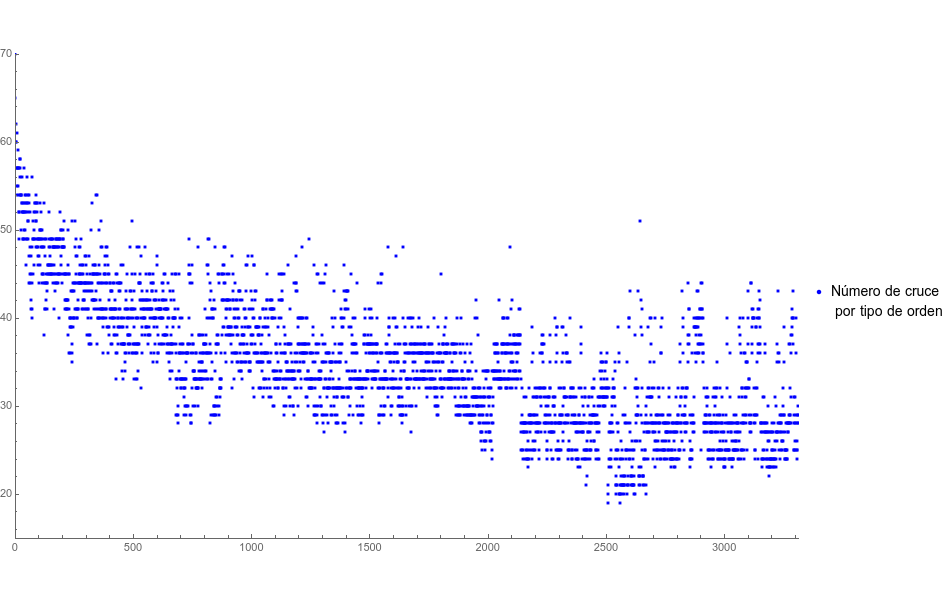
\includegraphics[width=1\linewidth]{exportP1_single}
      \caption{Mostramos el resultado de ordenar los tipos de orden de acuerdo al número de thrackles máximos. Graficamos etiquetas de los tipos de orden contra el número de cruce.}
      \label{fig:cnk8}
    \end{figure}
    \begin{figure}
      \centering
      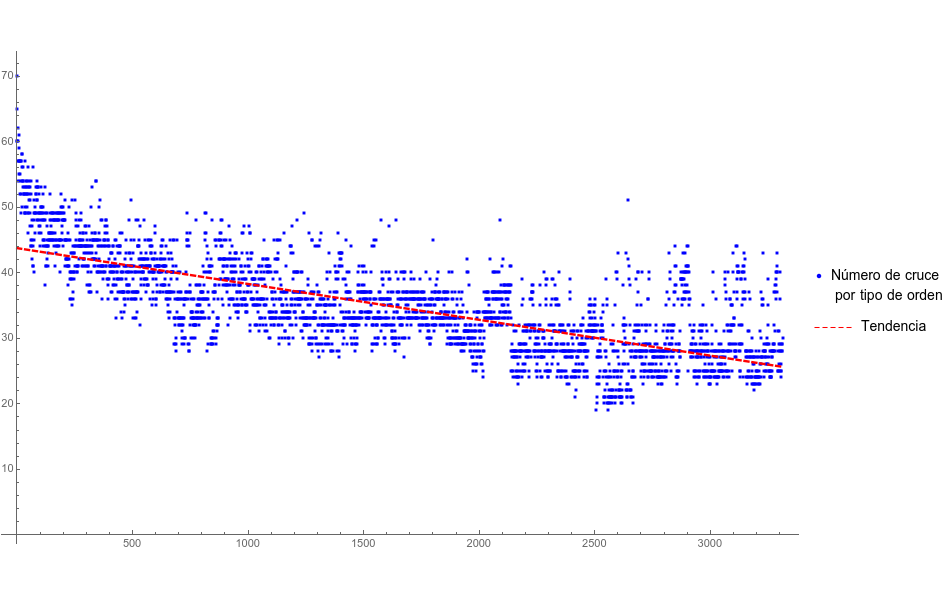
\includegraphics[width=1\linewidth]{exportP2}
      \caption{Mostramos la tendencia de los datos de la gráfica~\ref{fig:cnk8}, es posible observar que el número de thrackles máximos disminuye con respecto del número de cruce.}
      \label{fig:cnk8_2}
    \end{figure}
    Observamos también que los thrackles máximos que encontramos en los tipos de orden de 9
    vértices, de la tabla~\ref{table:res_desc_th_max} son ciclos de tamaño 3, con aristas con un
    extremo en vértices de grado uno y otro extremo en alguno de los vértices ápice del ciclo.

    Para cada $n$, con $n \in [3,10]$ listamos los tipos de orden, el número de thrackles máximos en
    cada tipo de orden y el número de cruce para cada tipo de orden. Estas listas están ordenados de
    acuerdo al número de thrackles en el tipo de orden de mayor a menor y pueden ser descargadas en
    la liga~\ref{link-thrMax_k} del apéndice~\ref{apendice-ligas}. Con este orden también notamos
    que el número de thrackles máximos disminuye casi de la misma manera que el número de cruce.

    En esta tesis decidimos analizar qué pasa con el anti-thickness de los tipos de orden en los que
    no existe ni un thrackle máximo, para esto usamos un algoritmo que encuentra, de manera
    exhaustiva, el anti-thickness de un dibujo dado. Explicamos este resultado a continuación.

\section{Anti-thickness de gráficas geométricas sin thrackles máximos}

  Una vez que obtuvimos el anti-thickness geométrico exacto para gráficas completas con hasta 10
  vértices, y al observar que podemos alcanzar este usando colecciones de thrackles máximos, nos
  preguntamos ¿cómo es el anti-thickness para los dibujos que no tienen thrackles máximos? ¿Es
  mayor? Y sí es así ¿cuánto más?

  En el trabajo de~\cite{Bulnes2017} se ofrece el número total de
  tipos de orden con hasta diez puntos, para los cuáles no existen thrackles máximos, en la
  tabla~\ref{tabla_totales} mostramos una comparación entre estos y el número de tipos de orden de
  $n$ para los cuales existe una descomposición por thrackles máximos con tamaño igual al
  anti-thickness de $K_n$. Es posible observar que si sumamos el número de tipos de orden sin
  thrackles máximos con el número de tipos de orden para los cuales existe una descomposición por
  thrackles máximos cuyo tamaño es igual al anti-thickness geométrico de $K_n$, aún queda un buen
  número de tipos de orden que analizar. Más del 60\% de tipos de orden con 8,9 y 10 puntos están
  fuera de estas dos clasificaciones.

  \begin{table}
    \centering
    \begin{tabular}{|c|c|c|c|}
      \hline
      $n$     & \makecell{No. Tipos de orden sin\\ thrackles máximos} & \makecell{No. Tipos de orden con\\
      descomposición por \\ thrackles máximos} & Total \\ \hline
      8       &  1175     & 2 & $1,177$ $(35.50\%)$   \\ \hline
      9       &  53758    & 7 & \makecell{$53,765$\\$(33.85\%)$}  \\ \hline
      10      &  4654339  & 3 & \makecell{$4,654,342 $\\$(32.52\%)$}  \\ \hline
    \end{tabular}
    \caption{En esta tabla mostramos el número de tipos de orden sin thrackles máximos, el número
    de tipos de orden que tienen una descomposición por thrackles máximos con tamaño igual al
    anti-thickness geométrico de $K_n$ y además la suma de estos dos números comparado con el total
    de tipos de  orden para cada $n$.}
    \label{tabla_totales}
  \end{table}

  Para responder estas interrogantes desafortunadamente no es posible formar colecciones de
  thrackles máximos y evaluar la cobertura de aristas como hicimos anteriormente. Por esta razón
  construimos un algoritmo que encuentra el anti-thickness de un dibujo geométrico inducido por un
  conjunto de $n$ puntos. El algoritmo es recursivo y usa una técnica de \emph{backtracking}.
  Discutimos con más detalle el algoritmo en la sección~\ref{secc:anti-thickness-dibujo}.

  En teoría, este algoritmo puede encontrar el anti-thickness de cualquier dibujo, para cualquier
  $n \geq 3$, sin embargo, debido a su costo computacional que es $O(n^{2+2n})$, solamente hicimos
  experimentos para $n\leq 8$. Hacemos el análisis de complejidad del algoritmo en la
  sección~\ref{secc:anti-thickness-dibujo}. Utilizando el algoritmo~\ref{algo_kthrackles} para
  encontrar thrackles máximos descrito en la sección \ref{seccion_algoritmo_kthrackles} listamos
  cuáles son los tipos de orden que no tienen thrackles máximos. La lista de cada uno de los tipos
  de orden que cumplen con esta característica puede ser descargada de la
  liga~\ref{link-thrWithoutMax} del apéndice~\ref{apendice-ligas}.

  Por otra parte, utilizamos estos tipos de orden como entrada para el algoritmo de búsqueda de
  anti-thickness de un dibujo de la sección~\ref{secc:anti-thickness-dibujo}. Encontramos que estos
  dibujos tienen anti-thickness mayor, en uno, al anti-thickness geométrico de $K_n$.

  Recordemos que en el trabajo de~\cite{Araujo2005} definen:
  \[
  d(n) = \max\{\chi(D(S)): S\subset \mathbb{R}^2 \text{ está en posición general}, |S|=n\},
  \]
  y donde además prueban que :
  \begin{equation}\label{eq_dn}
  5\left\lfloor\frac{n}{7}\right\rfloor \leq d(n) \leq \min\left(n-2,n-\frac{1}{2}-\frac{\lfloor \lg \lg
  n\rfloor}{2}\right).
  \end{equation}

  Con nuestros resultados encontramos el valor exacto de $d(n)$ para
  $n\in\{3,4,5,6,7,8\}$. Recordemos que, dado un conjunto $S$ de $n$ puntos, el número cromático
  $\chi(D(S))$ busca minimizar el número de thrackles necesarios para dar una descomposición de $K_n(S)$ como explicamos en la sección~\ref{cap3}. En el caso de $K_8$, existe al menos un dibujo que necesita cinco thrackles para su descomposición, por ejemplo, el dibujo en posición convexa. Sin embargo, como existe al menos otro dibujo para el que se necesitan seis thrackles en su descomposición y como este número coincide con el de la cota superior de la ecuación~\ref{eq_dn}, cuando $n=8$, decimos que $d(8)=6$. El resultado $d(7)=5$ se sigue del trabajo  de~\cite{Araujo2005}. Para los valores de $d(n)$ con $n \in \{3,4,5,6\}$ verificamos que el máximo número de thrackles necesarios en una descomposición de $K_n$ es, en efecto, $n-2$. En la tabla~\ref{tabla_ds} mostramos, para cada $n \in \{3,4,5,6,7,8\}$ el número de uno de los tipos de orden que necesita exactamente $n-2$ thrackles en su descomposición. Encontramos que para
  todos los tipos de orden que inducen gráficas completas sin thrackles máximos se necesitan $n-2$
  thrackles máximos para dar una descomposición. Nosotros creemos que en efecto,
  $d(n)=min\left(n-2,n-\frac{1}{2}-\frac{\lfloor \lg \lg n\rfloor}{2}\right)$.
  \begin{table}
    \centering
    \begin{tabular}{|c|c|}
      \hline
      $n$ & Tipo de orden \\ \hline
      3   & 0 \\ \hline
      4   & 1 \\ \hline
      5   & 2 \\ \hline
      6   & 14 \\ \hline
      7   & 80 \\ \hline
      8   & 1943 \\ \hline
    \end{tabular}
    \caption{En los tipos de orden de $n$ listados se requiere de $n-2$ thrackles para dar una
    descomposición por thrackles. Nótese que estos tipos de orden inducen gráficas completas que no tienen
    thrackles máximos.}
    \label{tabla_ds}
  \end{table}

  Todos los números de tipo de orden de tamaño $n$, para $n \in [3,8]$, para los que se ejecutó el
  algoritmo y el anti-thickness encontrado para cada uno pueden descargarse desde la
  liga~\ref{link-thrWithoutMax-at} del apéndice~\ref{apendice-ligas}. Con lo anterior demostramos
  el siguiente teorema.
  \begin{theorem}
    \label{teo:at_sin_thracklesmax}
    El anti-thickness de los dibujos para los cuales no existen thrackles
    máximos es mayor o igual que el anti-thickness geométrico de $K_n$, con $n \in [3,10]$.
  \end{theorem}

  Encontramos también, que para $3 \leq n \leq 8$ los conjuntos de puntos que tienen $k$-convexidad
  alta, cuya definición establecimos en la sección~\ref{secc:descomposicion_thrackles_maximos},
  tienen anti-thickness mayor que el convexo por una unidad.

  En la siguiente sección analizamos, para $3 \leq n \leq 9$, cómo se comporta la intersección de
  thrackles, no necesariamente máximos, de los dibujos de $K_n$.

\section{Intersección de thrackles de $K_n$ con $3\leq n \leq 9$.}\label{secc:interseccion_thrackles}
    \chaptermark{Intersección de thrackles.}

    El teorema~\ref{teo:coleccion_optima} establecido en la sección
    ~\ref{secc:descomposicion_thrackles_maximos} nos indica que no existen colecciones óptimas de
    thrackles máximos que induzcan una descomposición por thrackles. Por ello, decidimos estudiar
    la existencia de colecciones de thrackles, no necesariamente máximos,
    cuya intersección a pares es vacía y que además puedan cubrir las aristas
    de $K_n$. Para explicar este proceso primero es necesario definir una
    \emph{partición de un entero}.

    \begin{definition}{\emph{Partición de un entero.}(~\cite{Knuth2011})}
      Una partición de un entero $n$ es una colección $P$ de enteros
      no negativos $\{a_1, a_2, \dots, a_m\}$ tales que
      $a_1 \geq a_2\geq \dots \geq a_m$ y $a_1 + a_2 + \dots + a_m = n$.
    \end{definition}
    %
    % Nosotros utilizamos las particiones de enteros como guía para construir una
    % descomposición y construimos un algoritmo que intenta encontrar dichas
    % descomposiciones en thrackles.

    Es posible usar ciertas particiones de un entero como guía para buscar
    descomposiciones en thrackles de $K_n$. Por ejemplo, si  deseamos obtener
    una descomposición en thrackles de $K_4$, entonces necesitamos cubrir
    seis aristas. El entero 6 tiene once particiones, tres de ellas son:
    $\{4,2\},\{2,2,2\},\{3,1,1,1\}$. Las cuales pueden traducirse a tres diferentes
    descomposiciones en thrackles, la partición $\{4,2\}$ se traduce en una descomposición
    con un thrackle con cuatro aristas y uno con dos aristas; la partición
    $\{2,2,2\}$ se traduce en una descomposición con tres thrackles con dos
    aristas cada uno; la partición $\{3,1,1,1\}$ se traduce a una descomposición
    con un thrackle con tres aristas y tres thrackles con una arista. Debido a que
    nosotros estudiamos descomposiciones de tamaño estrictamente menor
    a la cota superior del anti-thickness geométrico, que es
    $n - \left\lfloor\sqrt{2n+\frac{1}{4}} - \frac{1}{2}\right\rfloor$, y
    como en una descomposición solamente puede existir un thrackle máximo, es
    posible restringir el conjunto de particiones de enteros para
    las particiones que usaremos. Nos referimos a estas como
    \emph{particiones guía}.
    \begin{definition}{\emph{Partición guía.}} \label{definicion_particion_guia}
      Sea $K_n(S)$ la gráfica completa inducida por un conjunto $S$ de $n$
      puntos en posición general.
      Una partición $P=\{a_1,a_2,\dots,a_m\}$ es guía si cumple
      con las siguientes condiciones:
      \begin{itemize}
        \item Si $a_1$ es igual a $n$ entonces solo existe una ocurrencia de $a_1$ en $P$.
        \item La suma $a_1 + a_2 + \dots + a_m = \binom{n}{2}$.
        \item $m < n - \left\lfloor\sqrt{2n+\frac{1}{4}} - \frac{1}{2}\right\rfloor$.
      \end{itemize}
    \end{definition}

    No existe una fórmula cerrada para conocer el número de particiones de
    algún entero $n$. Una \emph{composición} de un entero $n$ es una partición
    en la que el orden de los elementos importa es decir, dos composiciones
    diferentes del entero 3 son $\{2,1\}$ y $\{1,2\}$. Podemos acotar el espacio de búsqueda de las
    particiones de un entero considerando únicamente las composiciones. Como el número de composiciones para un entero $n$ es $2^{n-1}$ podemos decir que existen a lo sumo $O(2^{n-1})$ particiones para el  mismo entero $n$.

    Usando la definición~\ref{definicion_particion_guia} generamos las particiones guía para todo entero
    $x\in \left\{ \binom{3}{2}, \binom{4}{2}, \dots, \binom{10}{2}\right\}$.
    En ~\cite{Knuth2011} se ofrece un algoritmo para
    generar las particiones de algún entero $n$. Nosotros utilizamos
    dicho algoritmo en este trabajo modificándolo para que genere solamente
    particiones guía de un entero. Discutimos con más detalle el algoritmo en
    la sección~\ref{secc:algo_particiones_validas}.
    La tabla~\ref{tabla:particionesk8k9} muestra las particiones generadas por el
    algoritmo. Nuestro algoritmo observó que para $x\in \left\{\binom{3}{2},\binom{4}{2}
    \cdots,\binom{7}{2}\right\}$ no existen particiones guía, esto reafirma,
    para $ 3\leq n\leq 7$, el resultado del teorema~\ref{teo:nuevacotainf}
    que establece una cota inferior para el anti-thickness geométrico de $K_n$. Por otro lado,
    no generamos las particiones para $K_{10}$ ya que debido al tamaño de los archivos binarios
    generados con el algoritmo de búsqueda de thrackles no fue posible diseñar un algoritmo con el
    mismo diseño de los discutidos en la sección~\ref{secc:algo_particiones_validas}. Esto es
    porque requerimos de cargar los archivos binarios a la memoria física para reducir las lecturas
    a disco, sin embargo los archivos relacionados con $K_10$ son demasiado grandes para la
    memoria. Una alternativa es partir los archivos en otros de menor tamaño pero esto
    incrementaria las lecturas a disco al cargar y descargar archivos a memoria y además requeriría
    que diseñaramos otra estrategia para estas tareas por lo que decidimos no examinar estos
    archivos.
    \begin{table}[t]
      \centering
      \begin{tabular}{|c|c|}
        \hline
        $n$                       & Particiones guía de $\displaystyle\binom{n}{2}$ \\ \hline\hline
        \multirow{2}{*}{$ 8 $}    & $\{8,7,7,6\}$ \\ \cline{2-2}
                                  & $\{7,7,7,7\}$ \\ \hline
        \multirow{11}{*}{$ 9 $}   &$\{9,8,8,8,3\}$ \\ \cline{2-2}
                                  &$\{9,8,8,7,4\}$ \\ \cline{2-2}
                                  &$\{9,8,8,6,5\}$ \\ \cline{2-2}
                                  &$\{9,8,7,7,5\}$ \\ \cline{2-2}
                                  &$\{9,8,7,6,6\}$ \\ \cline{2-2}
                                  &$\{9,7,7,7,6\}$ \\ \cline{2-2}
                                  &$\{8,8,8,8,4\}$ \\ \cline{2-2}
                                  &$\{8,8,8,7,5\}$ \\ \cline{2-2}
                                  &$\{8,8,8,6,6\}$ \\ \cline{2-2}
                                  &$\{8,8,7,7,6\}$ \\ \cline{2-2}
                                  &$\{8,7,7,7,7\}$ \\ \hline
      \end{tabular}
      \caption{Particiones de enteros del número de aristas de $K_8$ y de $K_9$. }
      \label{tabla:particionesk8k9}
    \end{table}

    Usando las particiones de la tabla~\ref{tabla:particionesk8k9} diseñamos
    una serie de algoritmos que buscan thrackles disjuntos usando estas particiones como guía.
    Como hay cerca de catorce algoritmos para realizar esta tarea, expondremos solamente
    uno de ellos en el algoritmo~\ref{algo:partition_decomposition} de la
    sección~\ref{secc:descomposiciones_particiones}, los
    otros algoritmos son similares a este. Como resultado de estos algoritmos podemos dar el
    siguiente teorema:
    \begin{theorem}\label{teorema:particiones}
      Sea $P=\{a_1,a_2,\dots,a_m\}$ una partición guía para $K_8$ o para $K_9$. No existe, para
      ningún dibujo diferente del convexo, una colección $\mathcal{D}=\{T_1,T_2,\dots,T_m\}$ de
      thrackles disjuntos tales que $|E(T_1)|=a_1,|E(T_2)|=a_2,\dots,|E(T_m)|=a_m$.
    \end{theorem}
    \begin{proof}
      Se sigue del resultado de la ejecución de los algoritmos para evaluar colecciones de
      thrackles. Los algoritmos encuentran que, para ninguna partición de la
      tabla~\ref{tabla:particionesk8k9}, existe una colección de thrackles disjuntos cuyo número de
      aristas corresponde a las particiones guía de $K_8$ y $K_9$.
    \end{proof}

    Estos resultados tienen implicaciones sobre la cota inferior del anti-thickness geométrico de
    $K_n$  para $n \in [3,9]$. Debido a que el número de elementos en las particiones guía es menor
    a  $n - \left\lfloor\sqrt{2n+\frac{1}{4}} - \frac{1}{2}\right\rfloor$ y como no encontramos
    ninguna  descomposición en thrackles usando alguna de las particiones guía, podemos concluir
    que el anti-thickness  geométrico de $K_n$ es mayor o igual a $n -
    \left\lfloor\sqrt{2n+\frac{1}{4}} -  \frac{1}{2}\right\rfloor$. Lo que confirma la discusión de
    la cota inferior en la sección~\ref{sec:cota_inf}.


\section{Algoritmos}\label{seccion_algoritmos}
  En esta sección presentamos los algoritmos usados en este trabajo. Empezamos
  describiendo el algoritmo para encontrar thrackles, de cualquier tamaño, dado
  un conjunto de puntos en posición general en el algoritmo~\ref{algo_kthrackles}. Después hablamos del algoritmo usado para encontrar la intersección de dos thrackles con el mismo número de
  aristas en el algoritmo~\ref{algo_interseccion}. Luego, explicamos el algoritmo que implementamos
  para encontrar colecciones de thrackles máximos de $K_n$ con el
  algoritmo~\ref{algo:descomposicion_thrackles_maximos}. Explicamos también como generamos las
  particiones guía de un entero con el algoritmo~\ref{algo:is_partition_valid} y como  usamos esas
  particiones para buscar colecciones de thrackles con un algoritmo exhaustivo en el
  algoritmo~\ref{algo:partition_decomposition}.
  Después, mostramos el algoritmo para encontrar el anti-thickness de un dibujo específico con el
  algoritmo~\ref{algo_exhaustive_at}. Finalmente, hablamos del algoritmo para calcular el número de
  cruce de un thrackle con el algoritmo~\ref{algo_cnthracklemax}.

  En la figura~\ref{fig:diagrama} explicamos cómo se relacionan los algoritmos con los resultados
  obtenidos. En esta figura ilustramos los resultados con rectángulos delineados continuamente y los
  algoritmos con rectángulos con lineas punteadas.

  \begin{figure}
    \centering
    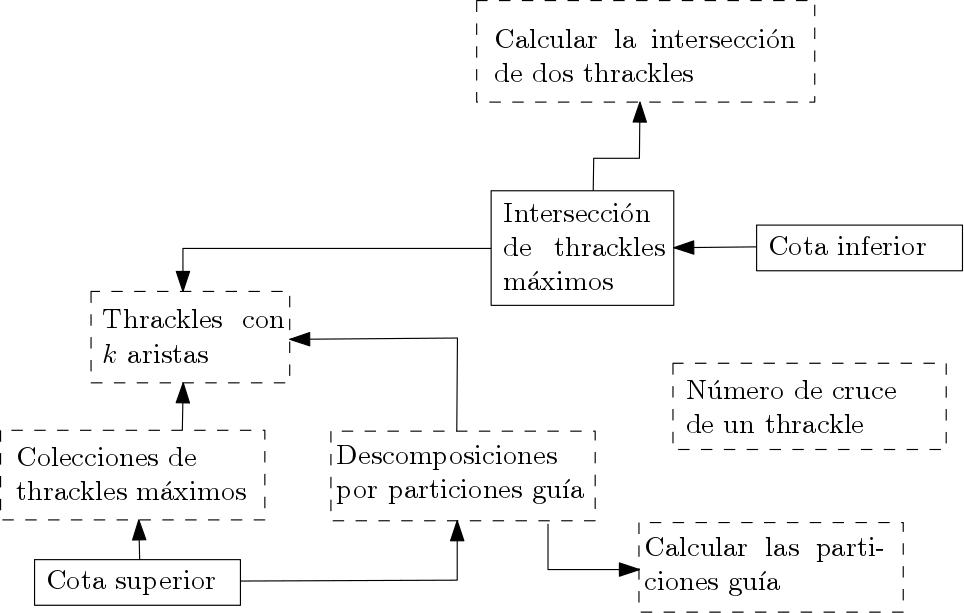
\includegraphics[width=0.9\linewidth]{diagrama}
    \caption{Ilustramos la relación entre algunos de los algoritmos y los resultados que describimos en esta tesis. Las flechas indican que algún resultado o algoritmo usó el resultado o el algoritmo al que está apuntado. Por ejemplo, el algoritmo de descomposiciones por particiones guía usa el algoritmo de búsqueda de thrackles con $k$ aristas y a su vez el resultado de dicho algoritmo está relacionado con la cota superior. Por otra parte, mejoramos la cota inferior del anti-thickness geométrico usando el resultado de la intersección entre thrackles máximos, para obtener este resultado buscamos los thrackles máximos para cada tipo de orden usando el algoritmo de búsqueda de thrackles con $k$ aristas.}
    \label{fig:diagrama}
  \end{figure}
  Los algoritmos fueron implementados en el lenguaje \texttt{C++} en su versión 5 (2017);
  las implementaciones fueron ejecutadas en un \emph{cluster} con las siguientes características:
  \begin{itemize}
    \item Procesador de 8 núcleos con velocidad de 1.5 GHz.
    \item Memoria RAM de 64 GB.
    \item Almacenamiento en disco duro de 128 GB.
  \end{itemize}
  Como nuestra implementación no está paralelizada, cada proceso corre en un solo procesador. Por lo que las comparaciones con el tiempo teórico son hechas tomando en cuenta solo un procesador de 1.5 GHz.

  Para almacenar información utilizamos, principalmente, una estructura de datos llamada vector. Un vector es un contenedor que representa a un arreglo que puede cambiar de tamaño. Podemos acceder al vector igual que se hace con un arreglo (usando el operador \texttt{[]}) con la misma complejidad.

\subsection{Algoritmo para encontrar thrackles con $k$
  aristas}\label{seccion_algoritmo_kthrackles}
  A continuación presentamos un algoritmo para resolver el siguiente problema:
  \begin{itemize}
    \item[] Problema: Dado $n$, deseamos encontrar todos los thrackles de tamaño $k$ de todas las gráficas completas $K_n(S)$, donde $S$ es un conjunto de $n$ puntos.
    \item[] Entrada: Un entero $n$, con $ 3 \leq n \leq 10$ y un entero $k$, con $ n \leq
    k$.
    \item[] Salida: Por cada tipo de orden de $n$ puntos, una lista de todos los thrackles de tamaño $k$ inducidos por el conjunto.
  \end{itemize}

  Este algoritmo requiere tres pasos de preparación para funcionar. Describimos estos pasos a continuación. Para cada tipo de orden $S$:
  \begin{enumerate}
    \item Leer y almacenar el archivo que contiene el tipo de orden $S$.
    Los puntos se almacenan en un vector de tamaño $n$ donde cada elemento es
    un objeto que contiene las coordenadas $x$ y $y$ de cada uno de los puntos
    de $S$.
    \item Generar y almacenar las aristas de la gráfica completa inducida por
    $S$. Para cada punto almacenado $p_i$, creamos todas las aristas (no
    dirigidas) que tienen como punto inicial a $p_i$ y como punto final a $p_j$,
    donde $ i+1 \leq j \leq n$.
    Las aristas son almacenadas en un vector de tamaño $\binom{n}{2}$ y las
    etiquetamos con enteros desde $0$ hasta $\binom{n}{2}-1$.
    \item \label{paso3}Construir la \emph{matriz de disyunción}.
    Construimos una matriz binaria de $\binom{n}{2}\times \binom{n}{2}$. La
    matriz es almacenada en un arreglo de arreglos convencional. Cada
    indice de las filas y de las columnas representa a cada una de las aristas
    de $K_n(S)$, de manera tal que la fila $i$ representa a la arista que tiene
    la etiqueta $i$, consideramos que la enumeración de las filas y columnas de
    la matriz empieza desde $0$, por lo que $i \in [0,\binom{n}{2}-1]$. Esto ocurre de la misma
    manera para las columnas.

    La matriz de disyunción tiene un 0 en la entrada $(i,j)$ si las aristas $i$ y $j$ se cruzan o
    comparten un vértice, y tiene un 1 en en la entrada $(i,j)$ si las aristas $i$ y $j$ son
    totalmente disjuntas. Es decir, construimos la matriz de adyacencia de la gráfica $D(S)$.
  \end{enumerate}

  A continuación describimos el algoritmo para encontrar thrackles
  de tamaño $k$, este algoritmo usa la matriz de disyunción construida en el
  paso~\ref{paso3} descrito anteriormente. El pseudocódigo se encuentra en el
  algoritmo~\ref{algo_kthrackles}.

  \begin{algorithm}[p]
      \DontPrintSemicolon
      \SetKwInOut{Input}{Entrada}
      \SetKwInOut{Output}{Salida}
      \underline{función EncontrarThrackle} $(n,k)$\;
      \Input{Un entero $n$, un entero $k$.}
      \Output{Una lista de thrackles de tamaño $k$ para cada tipo de orden de $n$.}
      Sea $C$ un vector de tamaño $k+1$;
      $C[0]\gets 0$\;
      $C[i]\gets NIL$ para $ 1 \leq i \leq k+1$\;
      %\State $C[1]\gets $
      \texttt{inters\_flag} $\gets$ \texttt{true}\;
      \texttt{curr\_size} $\gets 0$\;
      \While{$C[0] < \binom{n}{2}$}{
        \While{\texttt{curr\_size}$<k$}{
          \texttt{inters\_flag} $=$ \texttt{true}\;
          \If{$C[\text{\texttt{curr\_size}}] \geq \binom{n}{2}$}{
            \texttt{curr\_size} $\gets$  \texttt{curr\_size} $-1$\;
            \If{\texttt{curr\_size} $<0$}{
            \Return{Lista $L$ y \texttt{thrackle\_counter}}\;
            }
            $C[\text{\texttt{curr\_size}}]\gets C[\text{\texttt{curr\_size}}]+1$\;
            \textbf{continue}\;
          }
          \For{$i\gets 0 \dots \text{\texttt{curr\_size}}-1$}{
            \texttt{inters\_flag}=\texttt{inters\_flag} $\&\&$\;
            \texttt{matrix}$[C[i]][C\text{\texttt{curr\_size}}]$\;
          }
          \If{\texttt{inters\_flag} $==$ \texttt{False}}{
            $C[\text{\texttt{curr\_size}}] \gets C[\text{\texttt{curr\_size}}] + 1$\;
            \textbf{continue}\;
            }
          \Else{
            \If{\texttt{curr\_size}$+1==k$}{
              \texttt{thrackle\_counter} $\gets$ \texttt{thrackle\_counter} + 1\;
              Almacenar $C$ en una lista de vectores $L$.\;
              \textbf{continue}\;
              }
            }
            $C[\text{\texttt{curr\_size}}+1] \gets C[\text{\texttt{curr\_size}}] + 1$\;
        }
        \texttt{curr\_size} $\gets$ \texttt{curr\_size} $+1$\;
      }
      %\Return{$L$}
    \caption{Algoritmo para encontrar todos los thrackles de tamaño $k$.}
    \label{algo_kthrackles}
  \end{algorithm}

  El algoritmo que diseñamos utiliza la técnica de \emph{backtracking},
  recordemos que se desea encontrar todos los thrackles de tamaño $k$. Para
  nosotros, un solo thrackle de tamaño $k$ es una solución. Una solución es
  almacenada en un vector $C$. Almacenamos las etiquetas de las aristas que
  conforman un thrackle de tamaño $k$ en las entradas del vector.

  En cada iteración, el algoritmo verifica si ya se han encontrado $k$ aristas
  que se intersectan a pares, para evaluar la intersección se usa la matriz de
  disyunción.

  Supongamos que el vector $C$ tiene entradas desde $C[0]$ hasta $C[j]$ y que
  $j+1 < k$. Esto quiere decir que las aristas $C[0],C[1],\dots,C[j]$ forman un
  thrackle con $j+1$ aristas. El algoritmo buscaría extender el tamaño de este
  thrackle en uno. Para esto hacemos $C[j+1]=C[j]+1$ y verificamos si $C[j+1]$
  intersecta a $C[0],C[1],C[2],\dots,C[j-1],C[j]$. Si lo hace, entonces
  $C[j+1]$ forma parte del thrackle y ahora el thrackle tiene $j+2$ aristas. En
  caso contrario hacemos $C[j+1]=C[j+1]+1$, es decir, se descarta la arista que
  estaba en $C[j+1]$ y es reemplazada por la arista subsecuente en la
  etiquetación.

  Si en algún momento la entrada $C[j]$ tiene un valor mayor o igual a
  $\binom{n}{2}$, esto es, que ya agotó los valores posibles para representar
  alguna arista en $K_n$, entonces, se incrementa el valor de la entrada
  $C[j-1]$ en uno y se continua la verificación a partir de esta entrada. Esto
  permite que el algoritmo realice el proceso de \emph{backtracking}.

  Si el vector $C$ tiene $k$ entradas, es decir, encontró un thrackle con $k$
  aristas entonces almacenamos el contenido del vector $C$ en una lista de
  vectores. Como ya se encontró una solución y esta ha sido procesada, para
  buscar la siguiente solución, le indicamos al algoritmo que el thrackle tiene
  actualmente tamaño $k-1$, provocando así que en la siguiente iteración se
  busque incrementar el tamaño del thrackle en uno.

  Mostramos un ejemplo de cómo se llena el vector $C$ en una
  ejecución del algoritmo en la figura~\ref{fig:ejemplo_backtracking}.
  \begin{figure}[p]
    \centering
    \begin{tikzpicture}[
     node distance = 15mm and 1mm,
       start chain = A going right,
       start chain = R going right,
       nd/.style = {draw=none, fill=none, on chain=A, minimum width =10mm},
       mpn/.style args = {#1/#2/#3/#4}{draw,
       rectangle split, rectangle split horizontal,
       rectangle split parts=4,
       on chain=A,
       node contents={ \nodepart{one}    $#1$
                       \nodepart{two}    $#2$
                       \nodepart{three}  $#3$
                       \nodepart{four}   $#4$}
                                   },
       root/.style args = {#1/#2/#3/#4}{draw,
       rectangle split, rectangle split horizontal,
       rectangle split parts=4,
       on chain=R,
       node contents={ \nodepart{one}    $#1$
                       \nodepart{two}    $#2$
                       \nodepart{three}  $#3$
                       \nodepart{four}   $#4$}
                                   },
                           ]


       \node[mpn=0/NIL/NIL/NIL]; %A1
       \node[mpn=1/NIL/NIL/NIL]; %A2
       \node[mpn=2/NIL/NIL/NIL]; %A3
       \node[nd]{...};           %A4
       \node[mpn=0/1/NIL/NIL, below=of A-1];   %A5
       \node[mpn=0/2/NIL/NIL, right=of A-5]; %A6
       \node[mpn=0/1/2/NIL, below=of A-5 ]; %A7
       \node[nd,right=of A-6]{...}; %A8
       \node[mpn=0/1/3/NIL, right=of A-7];  %A9
       \node[mpn=0/1/3/4, below=of A-9, fill=gray]; %A10
       \node[mpn=0/1/3/5, right=of A-10, fill=gray]; %A11
       \node[nd,right=of A-11]{...}; %A12
       \node[nd, right=of A-6]{...}; %A13
        \node[nd, right=of A-9]{...}; %A14
        \node[nd, below=of A-4]{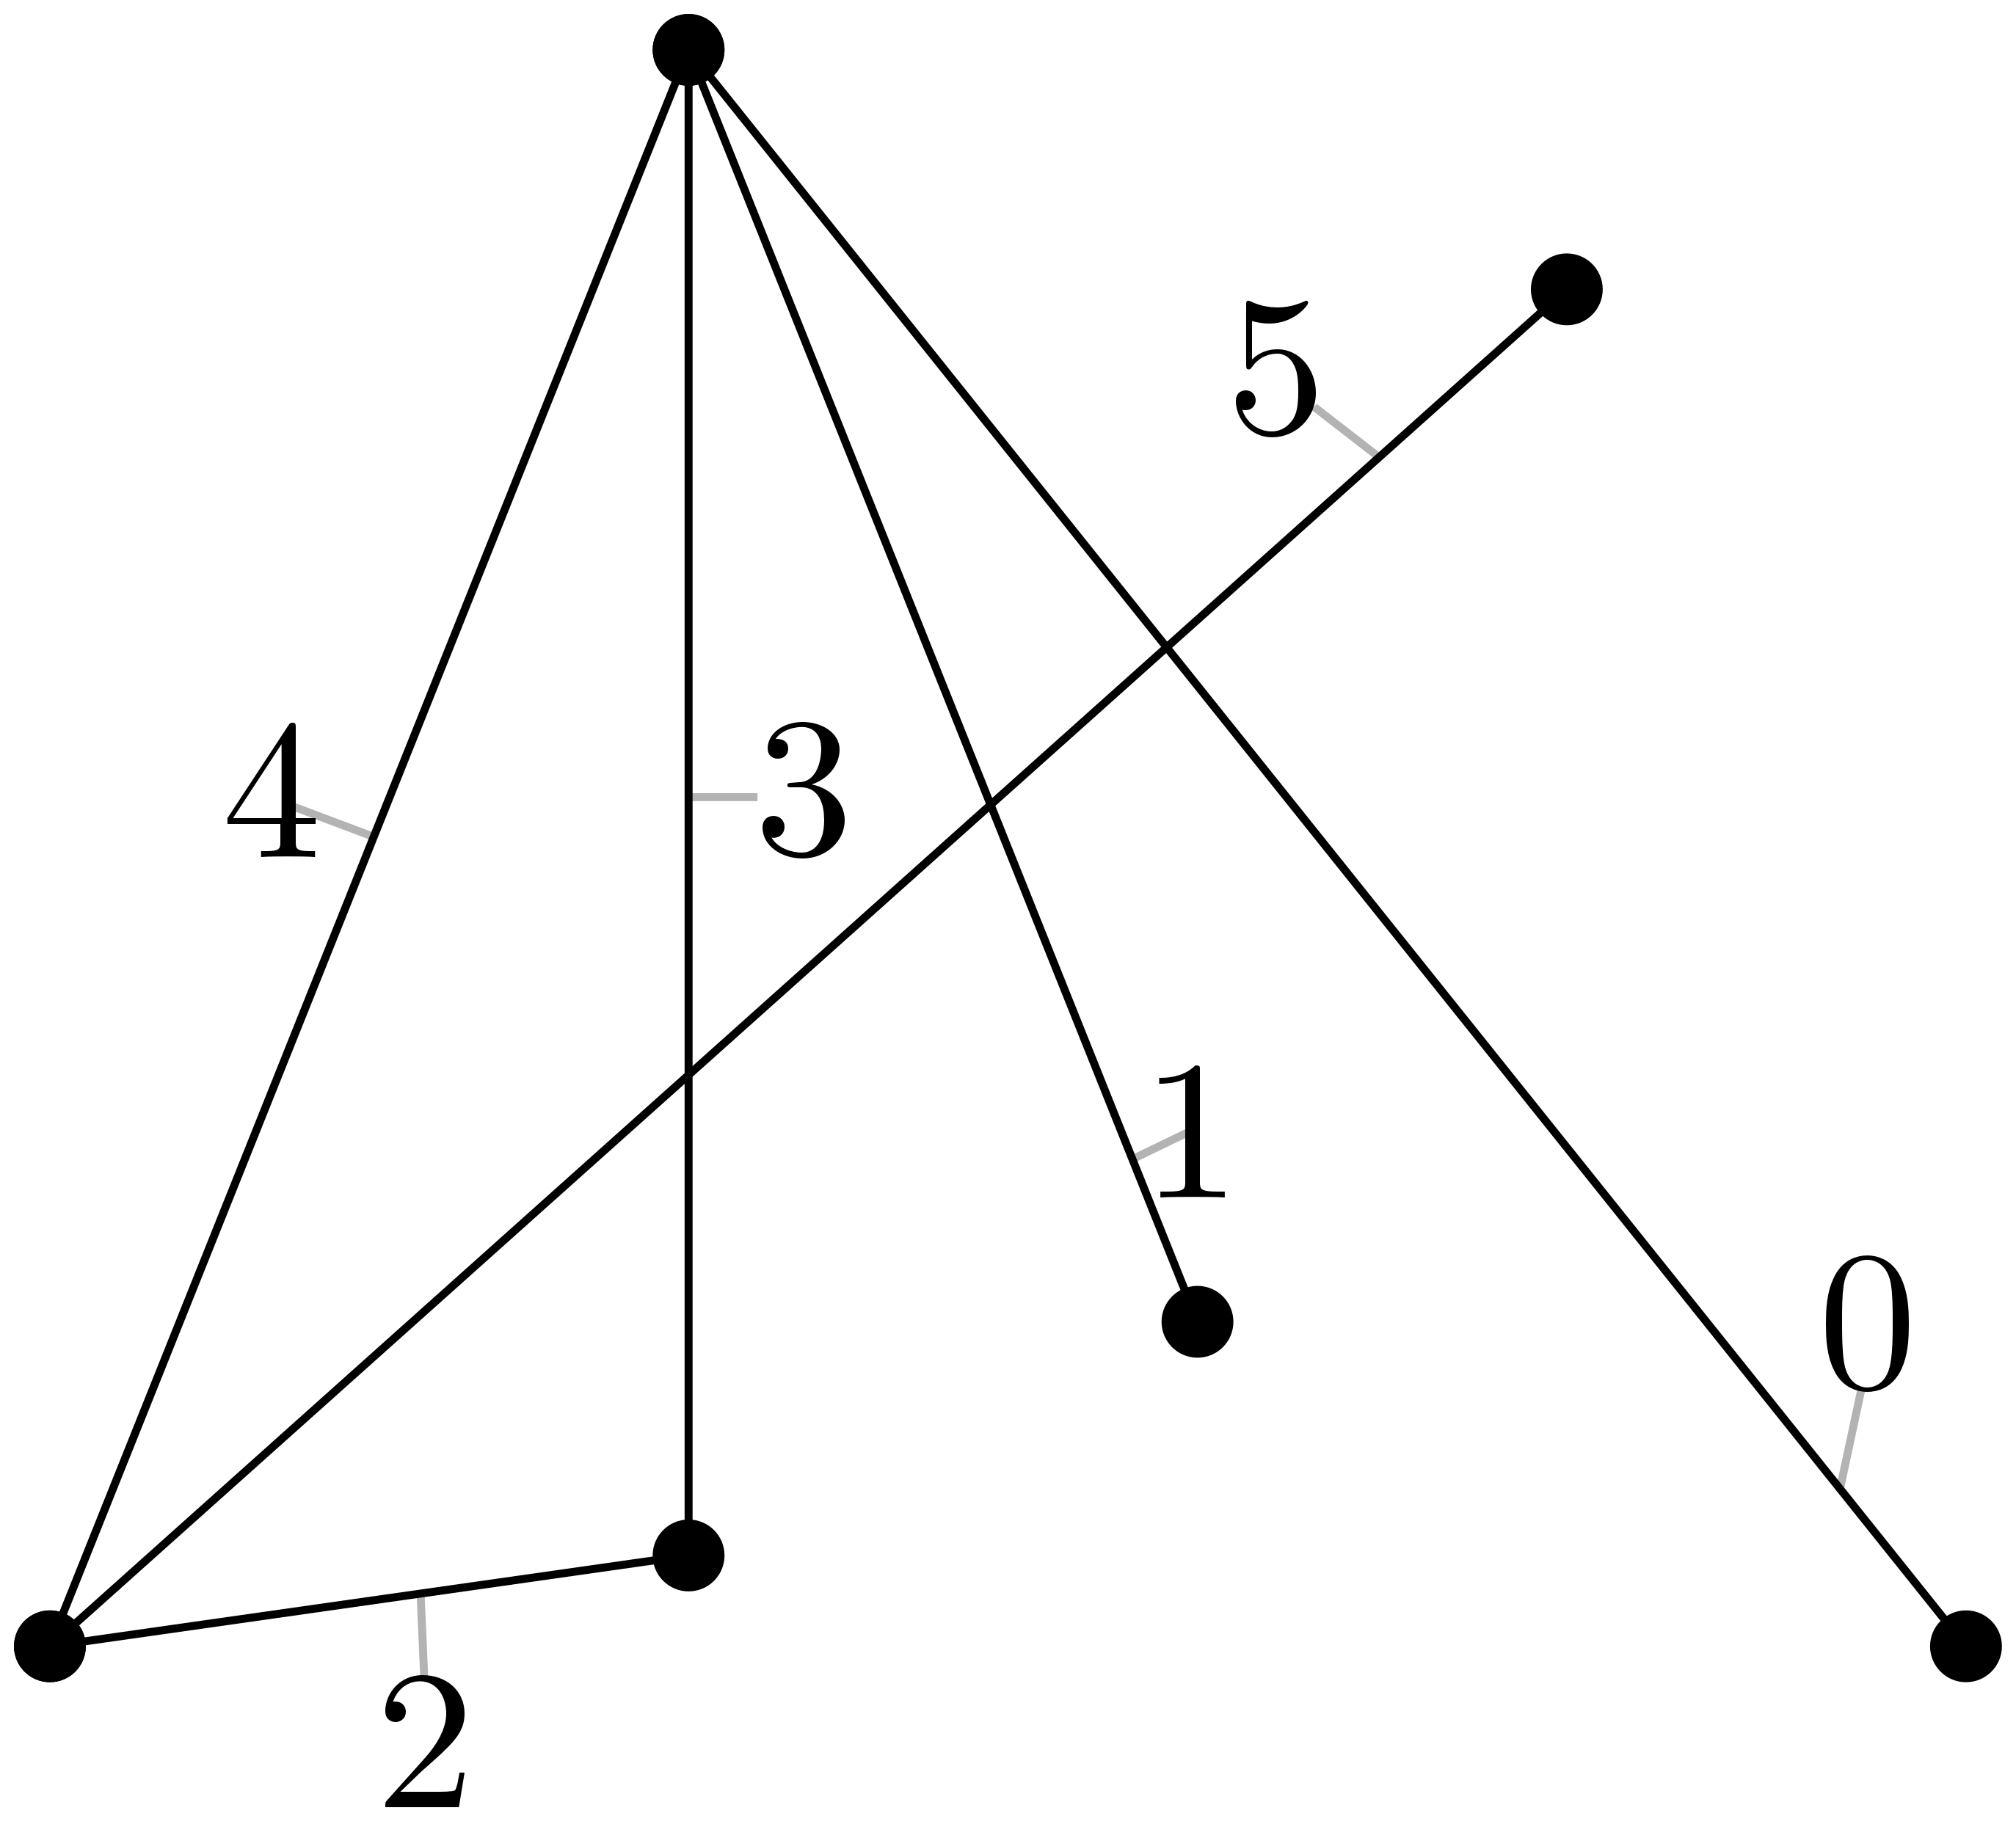
\includegraphics[width=0.4\textwidth]{ejemplo_backtracking}};
       %\draw{...}
       %
       \node[root=NIL/NIL/NIL/NIL, %ROOT.
             above=of $(A-1.north west)!0.5!(A-4.north east)$];

       \foreach \i in {1,...,3}
       \draw[-Stealth, semithick, shorten >=1mm, shorten <=1mm]
           (R-1.south) -- (A-\i.north);
       \draw[-Stealth, semithick, shorten >=1mm, shorten <=1mm]
           (R-1.south) -- (A-4.north);
       \draw[-Stealth, semithick, shorten >=1mm, shorten <=1mm]
           (A-1.south) -- (A-5.north);
       \draw[-Stealth, semithick, shorten >=1mm, shorten <=1mm]
           (A-1.south) -- (A-6.north);
       \draw[-Stealth, semithick, shorten >=1mm, shorten <=1mm]
           (A-1.south) -- (A-8.north);
       \draw[-Stealth, semithick, shorten >=1mm, shorten <=1mm]
           (A-5.south) -- (A-7.north);
       \draw[-Stealth, semithick, shorten >=1mm, shorten <=1mm]
           (A-5.south) -- (A-9.north);
       \draw[-Stealth, semithick, shorten >=1mm, shorten <=1mm]
           (A-5.south) -- (A-14.north);
       \draw[-Stealth, semithick, shorten >=1mm, shorten <=1mm]
           (A-9.south) -- (A-10.north);
       \draw[-Stealth, semithick, shorten >=1mm, shorten <=1mm]
           (A-9.south) -- (A-11.north);
       \draw[-Stealth, semithick, shorten >=1mm, shorten <=1mm]
           (A-9.south) -- (A-12.north);
    \end{tikzpicture}
    \caption{La figura muestra un ejemplo de cómo cambia el vector $C$ cuando se busca un thrackle
    con 4 aristas para alguna $n>5$. En el lado derecho presentamos un dibujo de una gráfica en la
    que se buscan los thrackles con 4 aristas. Solamente se representan algunas instancias del
    vector $C$. En este ejemplo suponemos que las aristas con etiqueta 1 y 2 no se
    intersectan. Es posible observar que cuando $C=[0,1,2,NIL]$ no se generan, debajo de ese nivel,
    combinaciones con las etiquetas 1 y 2. Se marcan de fondo gris las soluciones encontradas.
    }
    \label{fig:ejemplo_backtracking}
  \end{figure}
  En el  inicio de la ejecución del algoritmo, el vector $C$ está vacío, es
  decir, que  todas sus entradas tienen un valor nulo. Esto se representa en
  la raíz del árbol generado implícitamente por el backtracking. Podemos pensar que el
  árbol implícito se construye primero a profundiad, similar a un recorrido de búsqueda
  en profundidad (DFS). El primer subárbol que se genera, después de la raíz, es aquel
  cuya raíz tiene a $C[0]=0$ y las demás posiciones con un valor nulo, llamemosle $r_1$.
  Si aún no se alcanza el tamaño de thrackle deseado, después generamos, como hijo de
  $r_1$, el subárbol cuya raíz tiene a $C[0]=0$ y $C[1]=1$ y las demás posiciones con un
  valor nulo, llamemosle $r_2$. Si aún no se alcanza el tamaño de thrackle deseado,
  después generamos, como hijo de $r_2$, el subárbol cuya raíz tiene a $C[0]=0,C[1]=1$ y
  $C[2]=2$ y las demás posiciones con un valor nulo. Repetimos este proceso hasta que
  alcancemos el tamaño de thrackle que buscamos. Cada nodo genera un hijo siempre y
  cuando las aristas representadas en $C$ se intersecten a pares. En la figura
  ~\ref{fig:ejemplo_backtracking} mostramos un ejemplo de un árbol generado por el
  algoritmo que tiene 4 niveles.

  En la primera iteración hacemos $C[0] = 0$. Esta inicialización es necesaria para poner
  en marcha el algoritmo. De esta manera, el algoritmo encuentra primero todos
  los thrackles que contengan a la arista con etiqueta 0 en la primera posición. Una vez que la posición $C[0]$ tenga un valor mayor o igual a $\binom{n}{2}$, el valor de
  $C[0]$ será igual a 1. Esto hará que el algoritmo busque los thrackles que
  contengan a la arista con etiqueta 1 en la primera posición. Este proceso se repite para todos los valores entre $0$ y $\binom{n}{2}-1$.
  % Esto es representado por los nodos del nivel 1  del arbol. Después, para cada nodo $i$ en el nivel 1 del arbol, se generan los nodos
  % que representan un thrackle con las aristas de $i$ y la arista subsecuente en la etiquetación con respecto de la última arista de $i$. Estos nodos conforman el nivel 2 del arbol.

  Este algoritmo solamente genera soluciones que son thrackles.
  Puesto que en $C$ solo se avanza a la siguiente posición
  cuando se encuentra que la arista de la posición actual intersecta a las
  aristas anteriormente establecidas. Además, el algoritmo genera todos los
  thrackles con $k$ aristas, si no lo hiciera significaría que no evaluó
  determinada combinación de aristas. Recordemos que las aristas están etiquetadas
  con enteros desde $0$ hasta $\binom{n}{2}-1$. Supongamos que existe un subconjunto
  $T=\{a_1,a_2,\dots,a_k\}$ de las etiquetas $\{0,1,2,\dots,\binom{n}{2}-1$ que
  representa un thrackle de tamaño $k$ y que el algoritmo no evaluó. Existe un subárbol
  cuya raíz, llamemosle $r_1$ tiene a $C[0]=a_1$ y, por consiguiente $r_1$, tiene como
  hijo al subárbol cuya raíz, llamemosle $r_2$ tiene a $C[0]=a_1$ y a $C[1]=a_2$ y así
  sucesivamente hasta llegar a un nodo sin hijos que tiene a $C[0]=a_1,C[1]=a_2,\dots
  C[k]=a_k$, si el algoritmo no evaluó esta combinación, significa que no generó alguno
  de los subárboles, en la línea 25 del algoritmo, que tienen como descendiente al nodo
  $C[0]=a_1,C[1]=a_2,\dots C[k]=a_k$ y esto sucede cuando existe al menos un par de
  aristas $a_i,a_j\in T$ que son  disjuntas. Esto contradice la suposición de que $T$
  representa un thrackle, por lo tanto, si $T$ es un thrackle, entonces el algoritmo lo
  evalúa, esto sucede en el ciclo \texttt{for} de la línea 15.

  Para el caso particular de la entrada $C[0]$, se toman los valores en el rango $\left[ 0, \binom{n}{2}\right]$. Las combinaciones que se descartan, al hacer la evaluación en la línea 18, son aquellas que no forman un thrackle, estas son las combinaciones que contienen al menos una arista disjunta de alguna de las otras aristas de la combinación.

  \subsubsection{Análisis de complejidad}
  El caso en el que este algoritmo realiza más cálculos es aquel en el que no se descarta ninguna combinación de tamaño $t$ para $t \leq k$ y por lo tanto el algoritmo analiza, en tiempo $O(t)$, cada combinación en el ciclo de la línea 15. Para establecer el costo computacional del algoritmo es necesario saber cuántas combinaciones de tamaño $t$ existen para cada $t\leq k$ y multiplicar esto por el costo de evaluar cada combinación. Como hay $\binom{n}{2}$ aristas y estamos suponiendo que cualquier combinación de tamaño $t$ es válida, existen $\displaystyle \binom{\binom{n}{2}}{t}$ combinaciones de dicho tamaño. Se necesitan $\displaystyle t \binom{\binom{n}{2}}{t}$ operaciones para evaluar todas las combinaciones de tamaño  $t$. En nuestro caso $ t \in [1,10]$, por lo tanto el costo computacional del algoritmo, en el peor caso es:
  \begin{dmath}
    \displaystyle O\left( \sum_{t=1}^{10} t\binom{\binom{n}{2}}{t} \right) =
    O\left(\binom{\binom{n}{2}}{1} + 2\binom{\binom{n}{2}}{2} + 3\binom{\binom{n}{2}}{3} +\dots+ 10\binom{\binom{n}{2}}{10} \right) = O(n^2)+ O(n^4)+ O(n^6) + \dots + O(n^{20}) = O(n^{20}),
    % \frac{563}{1260}n^2 - \frac{2009}{2880}n^3
    % -\frac{104929}{1451520}n^4 + \frac{942563}{2903040}n^5 + \frac{240847}{1548288}n^6 -
    % \frac{1819243}{11612160}n^7 -\frac{243803}{6635520}n^8 + \frac{35789}{1032192}n^9 +
    % \frac{2698441}{371589120}n^{10} - \frac{1048709}{185794560}n^{11} -\frac{26651}{41287680}n^{12}
    % + \frac{8717}{15482880}n^{13} + \frac{19}{589824}n^{14} - \frac{n^{16}}{6193152} +
    % \frac{11}{7741440}n^{17} -\frac{n^{18}}{13762560} - \frac{n^{19}}{37158912} +
    % \frac{n^{20}}{371589120} = O(n^{20}),
  \end{dmath}
   para cada tipo de orden de $n$ puntos.

   En teoría, el tiempo que necesitaríamos para ejecutar este algoritmo en el cluster es significativo. En la tabla~\ref{tabla:kthrackles_tiempo}, mostramos cuánto tiempo es requerido por este algoritmo con complejidad $O(n^{20})$ tomando en cuenta la velocidad de procesamiento del cluster. También mostramos cuánto tiempo tardó su ejecución para $n=\{8,9,10\}$.
   \begin{table}
     \centering
     \begin{tabular}{|c|c|c|}
       \hline
       $n$      & Tiempo teórico en cluster & Tiempo real en cluster \\ \hline
       10       &     2113.99 años          & 3 días \\   \hline
       9        &     257.01 años           & 12 minutos \\    \hline
       8        &     24.36 años            & 6 segundos \\  \hline
     \end{tabular}
     \caption{Tiempo de ejecución teórico del algoritmo y tiempo real de ejecución en el cluster.}
     \label{tabla:kthrackles_tiempo}
   \end{table}

     %\huge FALTA COMPARACIÓN CON MUNDO REAL}

  Los datos de los thrackles máximos encontrados para cada $ 3\leq n \leq 9$
  pueden ser descargados de la siguiente liga:
  \url{http://computacion.cs.cinvestav.mx/~dmerinos/site/archivos_tesis/3to9.tar.gz}
  el archivo para $n=10$, separado debido a su tamaño,
   puede ser descargado de la siguiente liga:
  \url{http://computacion.cs.cinvestav.mx/~dmerinos/site/archivos_tesis/10.tar.gz}

\subsection{Algoritmo para la intersección de dos thrackles}\label{secc:algo_interseccion_thrackles}
  Dados dos thrackles con el mismo número de aristas, con un arreglo de enteros que
  represente a sus aristas, aprovechamos el ordenamiento lexicográfico para hacer la
  operación de intersección de thrackles en tiempo lineal.
  Sea $A$ y $B$ dos vectores que representan las aristas de dos thrackles, con
  $|A|=|B|=k$. El algoritmo~\ref{algo_interseccion} entrega la intersección de $A$ y $B$
  y la almacena en un conjunto $C$. Este algoritmo es secuencial y visita en el peor caso
  todas las entradas de los dos vectores, en nuestra implementación, los thrackles
  almacenan la información de sus aristas en un vector de tamaño $\binom{n}{2}$ para cada
  $n$ en el rango $[3,10]$.
  \begin{algorithm}[]
    \DontPrintSemicolon
    \SetKwInOut{Input}{Entrada}
    \SetKwInOut{Output}{Salida}
    \underline{función Intersection} $(A,B,C)$\;
    \Input{Dos conjuntos $A,B$ del mismo tamaño y un conjunto $C$}
    \Output{Un conjunto $C$ con la intersección de $A$ y $B$}
      $i\gets 0$\;
      $j\gets 0$\;
      \While{$i<k$ and $j<k$}{
        \If{$A[i] < B[j]$}{
          $i\gets i+1$\;
          \textbf{continue}\;
        }
        \If{$A[i]==B[j]$}{
          $C\gets C\cup \{A[i]\}$\;
          $i\gets i+1$\;
          $j\gets j+1$\;
          \textbf{continue}\;
        }
        \If{$A[i]>B[j]$}{
          $j\gets j+1$\;
          \textbf{continue}\;
        }
      }
    \caption{Intersección de dos conjuntos ordenados en tiempo
    lineal.}
    \label{algo_interseccion}
  \end{algorithm}

\subsection{Algoritmo para encontrar colecciones de thrackles máximos de $K_n$} \label{secc:algo_descomposicion_thrackles_maximos}
  Aquí presentamos un algoritmo para resolver el siguiente problema:
  \begin{itemize}
    \item[] Problema: Para cada tipo de orden de $n$ puntos, con $3 \leq n \leq 10$, determinar si existen y, si es el caso, encontrar las colecciones de thrackles máximos que pueden inducir una descomposición de $K_n$.
    \item[] Entrada: Un entero $n$, con $ 3 \leq n \leq 10$.
    \item[] Salida: Para cada tipo de orden de $n$ puntos, una lista de colecciones de thrackles máximos que pueden inducir una descomposición de $K_n$.
  \end{itemize}

  El algoritmo que diseñamos para este resultado es exhaustivo y secuencial.

  Este algoritmo necesita un paso de preparación para funcionar: Para cada tipo de orden,
  para $3\leq n \leq 10$, examinamos cuáles tienen al menos $n - \left\lfloor\sqrt{2n +
  \frac{1}{4}} - \frac{1}{2}\right\rfloor$ thrackles máximos. De los resultantes,
  examinamos cuáles tipos de orden cubren, con la unión de sus thrackles máximos, todas
  las aristas de $K_n$.

  \begin{algorithm}[t]
    \DontPrintSemicolon
    \SetKwInOut{Input}{Entrada}
    \SetKwInOut{Output}{Salida}
    \underline{función FindThrackleCollections} $(n,ot)$\;
    \Input{Un entero $n$, un entero $ot$ que representa algún tipo de orden válido de
    $n$.}
    \Output{Las combinaciones de $At_g(K_n)$ thrackles máximos que pueden inducir una
    descomposición del dibujo de $K_n$ inducido por el tipo de orden $ot$.}
    $c \gets n - \left\lfloor\sqrt{2n + \frac{1}{4}} - \frac{1}{2}\right\rfloor$\;
    $\mathcal{T} \gets $ colección de thrackles máximos del tipo de orden $ot$\;
    $k \gets |\mathcal{T}|$\;
    $C \gets $ combinaciones de tamaño $c$ del conjunto $\{1,2,\dots,k\}$\;
    \ForEach{$t\in C$}{
      $solution \gets \{T[t[1]],T[t[2]],\dots,T[t[k]]\}$\;
      \If{$solution$ cubre las aristas de $K_n$}{
        Almacenar $solution$ en una lista de soluciones.
        }
      }
    \caption{Búsqueda de colecciones de thrackles máximos que inducen una descomposición
    de $K_n$}
    \label{algo:descomposicion_thrackles_maximos}
  \end{algorithm}

  Después de la etapa de preparación, podemos empezar la búsqueda de las colecciones de
  thrackles máximos. Mostramos el pseudocódigo en el
  algoritmo~\ref{algo:descomposicion_thrackles_maximos}. Una vez que sabemos cuáles son
  los tipos de orden candidatos a tener una colección de thrackles máximos que induzcan
  una descomposición de $K_n$, buscamos de manera exhaustiva todas las combinaciones
  posibles de $n -  \left\lfloor\sqrt{2n + \frac{1}{4}} - \frac{1}{2}\right\rfloor$
  thrackles máximos. En nuestro pseudocódigo el número de thrackles máximos para cierto
  tipo de orden es denotado por $k$. Para cada una de las combinaciones verificamos si esta cubre o no a las aristas de $K_n$. Si la combinación cubre, almacenamos las etiquetas en una lista
  de soluciones y examinamos la siguiente combinación. En caso contrario descartamos esa
  combinación y continuamos examinando.

  Las combinaciones fueron generadas usando el algoritmo descrito en~\cite{Knuth2011A}.
  Mostramos el pseudocódigo del algoritmo para generar las combinaciones en el algoritmo
  \ref{algo:knuth_combinaciones} en la página \pageref{algo:knuth_combinaciones}. Dado un
  entero $k$, si queremos generar las combinaciones de un conjunto con cardinalidad $c$, el
  algoritmo~\ref{algo:knuth_combinaciones} tiene complejidad de
  $O\left(\binom{k}{c}\right) = O(k^c)$.

  En nuestro trabajo, $c$ es fija para cada $n$ ya que hacemos $c = At_g(K_n)$.
  Recordemos que $At_g(K_n) = n - \left\lfloor\sqrt{2n+\frac{1}{4}} -
  \frac{1}{2}\right\rfloor$. Sin embargo, el número de thrackles máximos, $k$, depende de dos parámetros: uno es $n$ y el otro es el tipo de orden de tamaño $n$ con el que trabajemos. Por ejemplo, para $n=6$ el tipo de orden $1$ tiene $13$ thrackles máximos, por lo que buscaríamos generar las $\binom{13}{3}$ combinaciones. Por otro lado, el tipo de orden $7$ tiene $5$ thrackles
  máximos, por lo que buscaríamos generar las $\binom{5}{3}$ combinaciones. Esto tiene un
  impacto en la complejidad del algoritmo.

  Sea $\mathcal{C}=\{c_1,c_2,\dots,c_k\}$ una combinación generada por el algoritmo\ref{algo:knuth_combinaciones}. $c_i\in\mathcal{C}$ representa una etiqueta de un thrackle máximo. Recordemos que el algoritmo entrega, para cada tipo de orden de tamaño $n$, una lista
  $\{\mathcal{C}_1,\mathcal{C}_2,\dots,\mathcal{C}_j\}$, donde cada $\mathcal{C}_i$ es
  una colección de thrackles máximos que pueden inducir una descomposición de $K_n$. Por
  ejemplo, si $\mathcal{C}_j=\{23,45,99\}$ entonces $\mathcal{C}_j$ representa una
  colección de tres thrackles máximos, los cuales tienen etiquetas 23, 45 y 99
  respectivamente. Es posible buscar en el archivo generado por el
  algoritmo~\ref{algo_kthrackles}, que busca thrackles con $k$ aristas, el thrackle que
  corresponde con determinada etiqueta y realizar operaciones sobre este.

  Para cada combinación calculada, el algoritmo verifica si esta cubre o no a las aristas
  de $K_n$. Hacemos esta verficación con un algoritmo secuencial que recorre el arreglo
  de aristas de cada thrackle identificado por las etiquetas de la combinación. En
  nuestra implementación cada thrackle de $K_n$ tiene asociado un arreglo de
  $\binom{n}{2}$ posiciones.
  \begin{algorithm}[p]
    \DontPrintSemicolon
    \SetKwInOut{Input}{Entrada}
    \SetKwInOut{Output}{Salida}
    \underline{función KnuthCombinations} $(n,t)$\;
    \Input{Un entero $n$, un entero $t$ con $0 \leq t \leq n$}
    \Output{Las combinaciones de $t$ elementos de los $n$ números en el conjunto $0,1,2,\dots,n-1$.}
    \For{$j=1\dots t$}{
      $c[j] \gets j-1 $\;
      }
    $c[t+1] \gets n$\;
    $c[t+2] \gets 0$\;
    \textbf{L2: } \;
    Almacenar la combinación $c[t],c[t-1],\dots,c[0]$. \;
    $j \gets 1$ \;
    \While{$c[j]+1 == c[j+1]$}{
      $c[j] \gets j-1$\;
      $j \gets j+1$\;
    }
    \If{ $j>t$ }{ \textbf{return}\; }
    $c[j] \gets c[j]+1$ \;
    $goto$\textbf{ L2}\;
    \caption{Algoritmo de Knuth para generar las combinaciones de tamaño $t$ del conjunto $\{0,1,2,\dots,n-1\}$.}
    \label{algo:knuth_combinaciones}
  \end{algorithm}


  \subsubsection{Análisis de complejidad}
  Sea $x=n - \left\lfloor\sqrt{2n + \frac{1}{4}} - \frac{1}{2}\right\rfloor$ para un tipo de orden válido, es decir, un tipo de orden con al menos $x$ thrackles máximos, de tamaño $n$, con $k$ thrackles máximos, el algoritmo~\ref{algo:descomposicion_thrackles_maximos} genera las
  $\binom{k}{x}$ combinaciones y después, para cada una, examina, en tiempo $O(x \cdot n^2)$, si esta cubre o no a las aristas de $K_n$. Este algoritmo tiene complejidad, para un tipo de orden de $n$ puntos:
  \begin{equation}\displaystyle
    O\left(\binom{k}{x}\cdot x n^2 \right) = O \left( \binom{k}{n} n^3 \right) = O(k^n n^3).
    \label{complejidad_colecciones}
  \end{equation}

  Es importante notar que la complejidad establecida en la
  ecuación~\ref{complejidad_colecciones} es para un tipo de orden. Nosotros
  ejecutamos este algoritmo para cada tipo de orden válido. Para saber cuántos thrackles
  máximos hay en determinado tipo de orden usamos el algoritmo~\ref{algo_kthrackles} descrito en la
  sección~\ref{seccion_algoritmo_kthrackles}. En la
  tabla~\ref{tabla:numero_operaciones_thrackles_maximos} damos un panorama de los valores que toma
  $k$ para $6\leq n \leq 10$. Con esto ilustramos también los valores que toma
  $displaystyle \binom{k}{x}$, es decir, el número de  combinaciones a evaluar por el algoritmo en el
  peor caso.

  \begin{table}
    \centering
    \begin{tabular}{|c|c|c|l|}
      \hline
      $n$ & \makecell{Número máximo de \\ thrackles en un T.O.} &$At_g(K_n)$& \makecell{Número de \\      combinaciones} \\
      \hline
      6 & 5 & 3 & 10 \\ \hline
      7 & 16 & 4 & 1,820 \\\hline
      8 & 49 & 5 & 1,906,884 \\\hline
      9 & 134 & 6 & 7,177,979,809 \\\hline
      10 & 333 & 6 & 1,809,928,822,548 \\ \hline
    \end{tabular}
    \caption{Se cuantifica el número de combinaciones a examinar por el algoritmo para el
    tipo de orden válido con más thrackles de cada $ 3 \leq n \leq 10$. Para los casos de
    $n = \{3,4,5\}$ no existen tipos de orden diferentes al convexo tal que la unión de
    thrackles máximos cubra las aristas de $K_n$.}
    \label{tabla:numero_operaciones_thrackles_maximos}
  \end{table}

  A pesar de que la complejidad descrita por la ecuación~\ref{complejidad_colecciones} es bastante
  grande, en la ejecución que realizamos obtuvimos tiempos de ejecución aceptables para el trabajo.
  En la tabla ~\ref{tabla:tiempo_colecciones_thrackles} describimos el tiempo de ejecución
  necesario para los tipos de orden de tamaños $n=\{8,9,10\}$ que tiene el mayor número de thrackles
  máximos y no es el convexo, y el tiempo de ejecución que tomó analizar todos los tipos de orden
  válidos. Podemos notar que a pesar de que en el caso de $K_{10}$ hay aproximadamente $1.8E^{12}$
  combinaciones posibles para uno de los tipos de orden de $10$ puntos, el algoritmo termina en un
  tiempo considerable para nosotros. Esto ocurre porque no todas las combinaciones posibles cubren las
  aristas de la gráfica completa, el algoritmo descarta una combinación cuando ninguno de los
  thrackles máximos de la colección cubre alguna arista en particular.

  \begin{table}
    \begin{tabular}{|c|c|c|c|}
      \hline
      $n$ & $m$ & Tiempo de ejecución teórico & Tiempo de ejecución real \\ \hline
      8   & 94  &  $2\times 10^{450}$ años    &  0.70 segundos           \\ \hline
      9   & 213 &  $3\times 10^{193}$ años    &  25 minutos               \\ \hline
      10  & 459 &  $1.3 \times 10^{74}$ años  &  4 días y 2 horas          \\ \hline
    \end{tabular}
    \caption{Mostramos el tiempo de ejecución real del algoritmo para todos los tipos de orden. La segunda columna indica cuántos thrackles máximos hay en como máximo en algún tipo de orden válido para cada $n$. La tercera columna indica cuánto tiempo necesitaría para acabar, en el peor caso. La última columna indica cuánto tiempo se necesitó en realidad.}
    \label{tabla:tiempo_colecciones_thrackles}
  \end{table}


  % La implementación de este algoritmo fue ejecutada en el cluster. En la
  % tabla~\ref{tabla:tiempo_thrackles_maximos} presentamos el tiempo de ejecución en milisegundos
  % para cada $n$ con $6\leq n \leq 10$. Podemos notar que a pesar de que en el caso
  % de $K_{10}$ hay aproximadamente $1.8E^{12}$ combinaciones posibles para uno de los
  % tipos de orden de $10$ puntos, el algoritmo termina en un tiempo considerable para
  % nosotros.
  % \begin{table}
  %   \centering
  %   \begin{tabular}{|c|c|}
  %     \hline
  %     $n$ & Tiempo de ejecución \\ \hline \hline
  %     6   & 6 ms \\ \hline
  %     7   & 6 ms \\ \hline
  %     8   & 708 ms \\ \hline
  %     9   & 25 minutos \\ \hline
  %     10  & 4 días, 2 horas y 6 minutos \\ \hline
  %   \end{tabular}
  %   \caption{La tabla muestra cuánto tiempo tomó el algoritmo para calcular las colecciones de $n -
  %   \left\lfloor\sqrt{2n + \frac{1}{4}} - \frac{1}{2}\right\rfloor$ thrackles que inducen una descomposición $K_n$.}
  %   \label{tabla:tiempo_thrackles_maximos}
  % \end{table}

  \subsection{Algoritmo para generar particiones guía de un
  entero}\label{secc:algo_particiones_validas}

    El algoritmo proporcionado en~\cite{Knuth2011} genera las particiones de algún entero
    $n$ con $O(n^2)$ operaciones, mostramos el pseudocódigo en el
    algoritmo~\ref{algo:particiones}. Una vez que las particiones son generadas,
    examinamos aquellas que tengan menos de $n - \left\lfloor\sqrt{2n + \frac{1}{4}} -
    \frac{1}{2}\right\rfloor$ elementos y evaluamos si son válidas. Una partición $P$, de
    tamaño $n -\left\lfloor\sqrt{2n + \frac{1}{4}} - \frac{1}{2}\right\rfloor$, de $n$ es
    una \emph{partición guía} si 1) todo elemento de $P$ es menor o igual a $n$ y 2) si algún $p_i\in P$ es
    igual a $n$, entonces solamente hay una ocurrencia de $p_i$ en $P$.
    \begin{algorithm}[htpb]
      \DontPrintSemicolon
      \SetKwInOut{Input}{Entrada}
      \SetKwInOut{Output}{Salida}
      \underline{función KnuthPartitions} $(n)$\;
      \Input{Un entero $n$, con $n\geq 1$.}
      \Output{Las particiones $P=\{a_1,a_2,\dots,a_k\}$ del entero $n$, tal que $a_1 \geq
      a_2 \geq \dots \geq a_k\}$ y $a_1 + a_2 +\dots + a_k = n$.}
      \textbf{P1}. $a_0 \gets 0$, $m\gets 1$\;
      \textbf{P2}. $a_m \gets n$, $q \ gets m - [n=1]$\;
      \textbf{P3}. Almacenar la partición $\{a_1,a_2,\dots,a_k\}$.\;
      \If{$a_q \neq 2$}{ \textbf{goto P5} }
      \textbf{P4}. $a_q \gets 1$ $q \gets q-1$, $m \gets m+1$, $a_m \gets 1$.\;
      \textbf{goto P4}\;
      \textbf{P5}. \If{$q==0$}{\textbf{return}}
      \Else{
        $x \gets a_q - 1$ \;
        $a_q \gets x$ \;
        $n\gets m-q+1$\;
        $m\gets q+1$\;
      }
      \textbf{P6}. \If{$n \leq x$}{\textbf{goto P2}}
      \Else{
        $a_m \gets x$\;
        $m \gets m+1$\;
        $n \gets n-x$\;
        \textbf{goto P6}\;
      }
      \caption{Algoritmo de Knuth para generar las particiones de un entero $n$.}
      \label{algo:particiones}
    \end{algorithm}

    Nuestra función para evaluar si una partición es una partición guía consiste en visitar
    cada posición de un arreglo con a lo sumo $n - \left\lfloor\sqrt{2n + \frac{1}{4}} -
    \frac{1}{2}\right\rfloor$ elementos y verificar que solamente exista una ocurrencia
    de $n$. Mostramos el pseudocódigo en el algoritmo~\ref{algo:is_partition_valid}. Esta tarea
    requiere analizar, en tiempo $O(1)$ cada una de los elementos del arreglo, cuyo tamaño es
    $O(n)$, por ello la prueba tiene complejidad lineal. Esta función es usada por el
    algoritmo de generación de particiones guía.

    \begin{algorithm}[htpb]
      \DontPrintSemicolon
      \SetKwInOut{Input}{Entrada}
      \SetKwInOut{Output}{Salida}
      \underline{función ParticionValida} $(n,P)$\;
       \Input{Un entero $n$, una partición $P$ de $n$ de tamaño $k$.}
       \Output{$true$, si la partición $P$ es válida, $false$ en otro caso.}
        $c \gets 0$\;
        \ForEach{$i \in P$}{
        \If{ $i > n$ }{ \Return{$false$}}
        \If{ $i == n$}{ $c \gets c+1$ }
        \If{$ c > 1 $}{ \Return {$false$}}
        }
        \Return{$true$}
       \caption{Algoritmo para evaluar si una partición es válida o no.}
       \label{algo:is_partition_valid}
    \end{algorithm}
    \subsubsection{Análisis de complejidad}

    El algoritmo para generar las particiones de un entero $n$ tiene complejidad
    $O(n^2)$. Adicionalmente, nosotros verificamos que las particiones  tengan
    menos de $n - \left\lfloor\sqrt{2n + \frac{1}{4}} - \frac{1}{2}\right\rfloor$
    elementos en tiempo lineal. Luego, para cada partición con el tamaño deseado,
    evaluamos si es válida o no. El costo total de este algoritmo es:
    \[ O(n^2\cdot n \cdot n) = O(n^4)\]

    La razón principal por las que definimos las particiones guía es porque pueden ser utilizadas
    como guía para buscar descomposiciones de $K_n$ donde cada elemento de la partición indica
    el tamaño de un thrackle. A continuación presentamos cómo utilizamos estas particiones
    para construir una serie de algoritmos.

\subsection{Algoritmo para encontrar descomposiciones por thrackles de $K_n$
usando particiones guía}\label{secc:descomposiciones_particiones}

  Este algoritmo fue diseñado para resolver el siguiente problema:
  \begin{itemize}
    \item[] Problema: Dada una partición $P=\{a_1,a_2,\dots,a_m\}$ de un entero $n$ con
    $m < At_g(K_n)$, deseamos encontrar si existe, para algún dibujo de $n$, una colección
    $\mathcal{C}=\{T_1,T_2,\dots,T_m\}$ de thrackles disjuntos tales que $|E(T_i)| = a_i$.
    \item[] Entrada: Una partición guía $P$ de $n$.
    \item[] Salida: $true$ si existe una colección de thrackles con las características
    descritas en el problema. $false$ en otro caso.
  \end{itemize}

  Como resultado del algoritmo para encontrar particiones guía descrito en la sección
  \ref{secc:algo_particiones_validas}, tenemos una lista de particiones guía para
  $n\in\{8,9\}$ que presentamos en la tabla~\ref{tabla:particionesk8k9_2}. En esta función cargamos a memoria los datos de los thrackles. En el caso de $K_{10}$ los archivos de los
  thrackles máximos y thrackles con 9 aristas exceden el tamaño de la memoria del cluster, por ello
  las particiones de $n=10$ no fueron evaluadas en este trabajo.
  \begin{table}[t]
    \centering
    \begin{tabular}{|c|c|}
      \hline
      $n$                       & Particiones válidas de $\displaystyle\binom{n}{2}$ \\ \hline\hline
      \multirow{2}{*}{$ 8 $}    & $\{8,7,7,6\}$ \\ \cline{2-2}
                                & $\{7,7,7,7\}$ \\ \hline
      \multirow{11}{*}{$ 9 $}   &$\{9,8,8,8,3\}$ \\ \cline{2-2}
                                &$\{9,8,8,7,4\}$ \\ \cline{2-2}
                                &$\{9,8,8,6,5\}$ \\ \cline{2-2}
                                &$\{9,8,7,7,5\}$ \\ \cline{2-2}
                                &$\{9,8,7,6,6\}$ \\ \cline{2-2}
                                &$\{9,7,7,7,6\}$ \\ \cline{2-2}
                                &$\{8,8,8,8,4\}$ \\ \cline{2-2}
                                &$\{8,8,8,7,5\}$ \\ \cline{2-2}
                                &$\{8,8,8,6,6\}$ \\ \cline{2-2}
                                &$\{8,8,7,7,6\}$ \\ \cline{2-2}
                                &$\{8,7,7,7,7\}$ \\ \hline
    \end{tabular}
    \caption{Particiones de enteros del número de aristas de $K_8$ y de $K_9$. }
    \label{tabla:particionesk8k9_2}
  \end{table}

  A continuación presentamos, con un caso particular, el esquema general de los
  algoritmos usados para verificar si existen colecciones de thrackles cuyos tamaños
  correspondan a los elementos de una partición. Este algoritmo utiliza la técnica de
  \emph{backtracking}, presentamos el pseudocódigo en el
  algoritmo~\ref{algo:partition_decomposition}.
  \begin{algorithm}[htpb]
    \LinesNumbered
    % This is to hide end and get the last vertical line straight
    \SetKwBlock{Begin}{Begin}{}
    \SetAlgoLined
    \DontPrintSemicolon
    \SetKwInOut{Input}{Entrada}
    \SetKwInOut{Output}{Salida}
    \SetKwProg{Forcut}{foreach}{}{}
    \underline{función 8876} $(n,P)$\;
     \Input{Un entero $n$, Una partición guía $P$ de $n$ de tamaño $k$.}
     \Output{$true$, si existe una colección de thrackles disjuntos en la que los tamaños de los thrackles corresponden a los elementos de $P$; $false$ en otro caso.}
     \Begin{
     Sea $Z$ un vector booleano de 28 posiciones.
     \For{$i\gets 0 \dots 28$}{
      $Z[i]=0$\;
     }
     Almacenar el estado actual de $Z$ en el arreglo $Z_1$.\;
     \ForEach{Thrackle $A$ de tamaño 8}{
        Sea $A.bedges$ el vector booleano  que representa las aristas de $A$.\;
        \For{$i \gets 0 \dots 26$}{
          \If{$A.bedges[i] == 1$}{
            \If{$Z[i] == 1$}{ % POSICIÓN OCUPADA THRACKLE NO DISJUNTO
              Restaurar $Z$ a $Z_1$.\;
              Descartar thrackle actual y continuar con el siguiente de tamaño 8.\;
            }
            \Else{
              $Z[i] \gets 1$\;
            }
          }
        }
        Almacenar el estado actual de $Z$ en el arreglo $Z_2$.\;
        \Forcut{Thrackle $B$ de tamaño 7}{
          Sea $B.bedges$ el vector booleano  que representa las aristas de $B$.\;
          \For{$i \gets 0 \dots 26$}{
            \If{$B.bedges[i] == 1$}{
              \If{$Z[i] == 1$}{ % POSICIÓN OCUPADA THRACKLE NO DISJUNTO
                Restaurar $Z$ a $Z_2$.\;
                Descartar thrackle actual y continuar con el siguiente de tamaño 7.\;
              }
              \Else{
                $Z[i] \gets 1$\;
              }
            }
          }
        }
     }
     }
     \caption{Algoritmo para buscar una colección de thrackles disjuntos de $K_n$ dada una partición guía de $n$.}
     \label{algo:partition_decomposition}
  \end{algorithm}

  \begin{algorithm}
    \LinesNumbered
    \setcounter{AlgoLine}{35}
    \SetKwBlock{Begin}{}{end}
    \Begin{
    Almacenar el estado actual de $Z$ en el arreglo $Z_3$.\;
    \ForEach{Thrackle $C$ de tamaño 7}{
      Sea $C.bedges$ el vector booleano  que representa las aristas de $C$.\;
      \For{$i \gets 0 \dots 26$}{
        \If{$C.bedges[i] == 1$}{
          \If{$Z[i] == 1$}{ % POSICIÓN OCUPADA THRACKLE NO DISJUNTO
            Restaurar $Z$ a $Z_3$.\;
            Descartar thrackle actual y continuar con el siguiente de tamaño 7.\;
          }
          \Else{
            $Z[i] \gets 1$\;
          }
        }
      }
      Almacenar el estado actual de $Z$ en el arreglo $Z_4$.\;
      \ForEach{Thrackle $D$ de tamaño 6}{
        Sea $D.bedges$ el vector booleano  que representa las aristas de $D$.\;
        \For{$i \gets 0 \dots 26$}{
          \If{$D.bedges[i] == 1$}{
            \If{$Z[i] == 1$}{ % POSICIÓN OCUPADA THRACKLE NO DISJUNTO
              Restaurar $Z$ a $Z_4$.\;
              Descartar thrackle actual y continuar con el siguiente de tamaño 6.\;
            }
            \Else{
              $Z[i] \gets 1$\;
            }
          }
        }
      }
      }
      }
  \end{algorithm}

  Para el funcionamiento de este algoritmo es necesario tener los datos de los thrackles de cada
  tamaño indicado por la partición, Por ejemplo, si se trabaja con $n=8$ y la partición guía es
  $\{8,7,7,6\}$, se debe usar la función de búsqueda de thrackles con $k$ aristas descrita en
  la sección~\ref{seccion_algoritmo_kthrackles} para buscar los thrackles con ocho, siete y seis
  aristas. No es necesario tener dos archivos diferentes para cada uno de los dos thrackles de
  tamaño siete, es suficiente tener un archivo para cada tamaño diferente.

  Tomemos el caso de la primera partición de ocho, $P=\{8,7,7,6\}$, en este caso queremos
  verificar si existe o no una colección de cuatro thrackles, uno de tamaño ocho, dos de
  tamaño siete y uno de tamaño seis, tal que sean disjuntos a pares. Para buscar esta colección,
  podemos diseñar un algoritmo que evalúe exhaustivamente la intersección de cada
  thrackle $A$ de tamaño ocho, con cada thrackle $B$ de tamaño siete. Si existen $A$ y $B$
  disjuntos, verificamos que exista algún thrackle $C$ de tamaño siete que sea disjunto con
  $A$ y con $B$ y, finalmente, si existe, buscamos un thrackle $D$, de tamaño seis que sea
  disjunto con $A,B$ y $C$.

  Para verificar que los thrackles sean disjuntos, mantenemos un arreglo booleano $Z$ de
  $\binom{8}{2}$ posiciones. Cuando se analiza un thrackle $T$ de tamaño 8 recorremos el arreglo de
  aristas de $T$, cuyo tamaño es también $\binom{8}{2}$. Como $T$ tiene 8 aristas entonces el
  arreglo de aristas de $T$ tiene exactamente 8 posiciones con valor uno
  y el resto con valor cero. Para cada posición $p$ de $T$ cuyo valor sea uno, marcamos la misma
  posición en $Z$ con uno. Esto significa que el thrackle $T$ cubre a la arista $p$.

  Si en algún momento debemos marcar alguna posición $p$ del arreglo $Z$ y esta ya tiene un valor
  de uno, entonces un thrackle anteriormente analizado ya cubre esa arista y por lo tanto el
  thrackle que se está verificando actualmente no es disjunto con alguno anterior. Por lo tanto
  descartamos ese thrackle y continuamos verificando con el thrackle subsecuente del archivo.

  Si no encontramos ningún thrackle que sea disjunto con los anteriormente analizados, el
  algoritmo descarta el último thrackle que fue compatible con los demás y continúa con el
  siguiente del mismo tamaño del thrackle descartado.

  El algoritmo termina, retornando un valor $true$, cuando encuentra un thrackle con ocho
  aristas, dos con siete aristas y uno con seis aristas, que son disjuntos a pares o bien, cuando
  no hay más thrackles que analizar. En este último caso el algoritmo retorna un valor $false$. Este algoritmo evalúa en el peor caso todas las combinaciones posibles de cuatro
  thrackles con tamaños 8,7,7 y 6 respectivamente.

  % Como paso de preparación, este algoritmo requiere tener los datos de los thrackles de
  % tamaño $8,7,7$ y $6$ para $K_8$. Y de manera general sea $P=\{a_1,a_2,\dots,a_m\}$, una
  % partición válida de $n$, es necesario tener los datos de los thrackles de tamaño $a_i$,
  % con $a_i\in P$.

  En nuestra implementación, decidimos almacenar los datos de los thrackles en la memoria
  del cluster para que el acceso fuera mucho más rápido que leer repetitivamente los
  archivos creados por el algoritmo de búsqueda de thrackles con $k$ aristas presentado
  en la sección~\ref{seccion_algoritmo_kthrackles}.

  Para las particiones guía presentadas en la tabla~\ref{tabla:particionesk8k9_2}, en la
  algunos de los casos no fue necesario construir funciones que evaluaran toda la
  partición. Para el caso de $n=9$ y las particiones $\{9,8,8,8,3\}$, $\{9,8,8,7,4\}$, $\{9,8,8,6,5\}$
  construimos un algoritmo que verifica la existencia de una colección de thrackles de tamaños
  nueve, ocho y ocho ya que la secuencia $\{9,8,8\}$ se repite en los tres casos, encontramos que no existen tres thrackles con nueve, ocho y ocho arsitas respectivamente que sean disjuntos por lo que no fue necesario hacer un procedimiento para cada una de las tres secuencias mencionadas. Para las particiones $\{9,8,7,7,5\}$, $\{9,8,7,6,6\}$, $\{9,7,7,7,6\}$ construimos
  un algoritmo que verifica la existencia de una colección de thrackles de tamaños nueve, siete,
  siete, siete y seis. Para ninguna de estas particiones guía se encontraron los respectivos thrackles disjunto. Para el resto de las particiones guía de $n=9$ escribimos un algoritmo para
  cada una. Para las dos particiones guía de $n=9$ construimos dos algoritmos.

  Las funciones construidas permitieron dar el resultado del
  teorema~\ref{teorema:particiones} de la sección~\ref{secc:interseccion_thrackles}.
  Estas funciones pueden encontrarse en la siguiente liga:

  \url{https://github.com/demaseme/programas_tesis_rev3/tree/master/cpps}.

  \subsubsection{Análisis de complejidad}
  La complejidad de este algoritmo está dado por el número de thrackles de cada
  tamaño establecido por la partición. Si existen $k$ thrackles de tamaño 8, $m$
  thrackles de tamaño 7 y $q$ thrackles de tamaño 6, el algoritmo realiza $O(k\cdot
  m^2 \cdot q)$ operaciones. Nótese el exponente de $m$ en la complejidad, recordemos que
  la partición guía es $\{8,7,7,6\}$ esto implica que por cada thrackle de tamaño 7, verificaremos
  con cada uno de los otros thrackles de tamaño 7 y por ello debemos considerar $m\times m$ en la
  complejidad.

  De manera general para una partición guía $P=\{a_1,a_2,\dots,a_m\}$, si existen $t_i$
  thrackles de tamaño $a_i$, en el peor caso hay
  \begin{equation} \label{ti}
    \binom{n}{2}^n t_i=\displaystyle \binom{\binom{n}{2}}{a_i}
  \end{equation}
  thrackles de tamaño $a_i$. La ecuación~\ref{ti} alcanza su máximo cuando $a_i=n$. Por lo que
  un algoritmo exhaustivo como el aquí presentado que usa como partición guía una partición que tiene
  $m$ elementos tiene, en el peor caso, una complejidad de
  \[O\left(\binom{\binom{n}{2}}{n}^m\right) = O(n^{2nm}). \]

  Por otro lado~\ref{ti} se minimiza cuando $a_i=1$, por lo que el algoritmo tiene como mejor caso una complejidad de :
  \[\omega\left(\binom{\binom{n}{2}}{1}^m\right)= \omega\left( \binom{n}{2}^m\right)= \omega(n^{2m}).\]

\subsection{Algoritmo para encontrar el anti-thickness de un dibujo de
$K_n$}\label{secc:anti-thickness-dibujo}

  El algoritmo presentado en esta sección resuelve el siguiente problema:
  \begin{itemize}
    \item[] Problema: Dado un conjunto de $n$ puntos en posición general deseamos encontrar el
    anti-thickness de la gráfica geométrica completa inducida por el conjunto.
    \item[] Entrada: Un conjunto de $n$ puntos en posición general.
    \item[] Salida: El anti-thickness de la gráfica completa inducida por el conjunto de puntos.
  \end{itemize}

  Este es un algoritmo exhaustivo y recursivo que usa la técnica de backtracking para encontrar el
  anti-thickness de un dibujo de $K_n$. El algoritmo realiza esta tarea buscando colecciones de thrackles
  cuyo tamaño sea mínimo, como en la definición~\ref{definicion:at_dibujo} de anti-thickness de un dibujo
  presentado en la sección~\ref{secc:anti-thickness}.

  Este algoritmo construye, implícitamente, un árbol en el que cada nodo es un thrackle y un camino desde
  la raíz hasta algún nodo es una colección de thrackles. Una colección de thrackles es una descomposición
  si la intersección a pares de cada thrackle en la colección es vacía y si la unión de las aristas de
  todos los thrackles es igual al conjunto de aristas de $K_n$. Decimos que dos thrackles son compatibles
  si su intersección es vacía. En este árbol la raíz es el nivel cero, los hijos de la raíz son el nivel 1,
  los hijos de los hijos de la raíz son el nivel 2 y así sucesivamente. El algoritmo baja de nivel en el
  árbol cuando encuentra un thrackle compatible con el resto de los thrackles que ya están en la colección.

  El algoritmo busca el thrackle de mayor tamaño posible en cada llamada recursiva para intentar agregarlo
  a la colección. Para poder agregarlo debe ser disjunto con los thrackles que ya existan en la colección.
  El algoritmo termina cuando no puede encontrar más colecciones de thrackles que cubran la gráfica
  completa y que tenga tamaño mínimo o bien, cuando las colecciones que encuentra son más grandes que el
  anti-thickness encontrado actualmente.

  Este algoritmo requiere que se lean los puntos y se induzca la gráfica completa así como la inicialización
  de la matriz de disyunción de la misma que mencionamos en la sección~\ref{seccion_algoritmo_kthrackles}
  del algoritmo de búsqueda de thrackles con $k$ aristas.

  En el algoritmo representamos un thrackle con un vector de enteros que representan las etiquetas de las
  aristas que inducen al thrackle. El vector de enteros tiene valores desde $0$ hasta $\binom{n}{2}-1$ ya que este es el rango de etiquetación de las aristas de $K_n$.
  \begin{algorithm}[p]
    \DontPrintSemicolon
    \SetKwInOut{Input}{Entrada}
    \SetKwInOut{Output}{Salida}
    \underline{función} exhaustive\_at $ (current\_thrackle,LevelAt) $\;
    \Input{Un vector de enteros que representa las aristas de un thrackle, un entero que representa el
    tamaño de la colección de thrackles actual.}
    \Output{El anti-thickness de la gráfica completa inducida por un conjunto de puntos.}
    \If{ $LevelAt \geq minAt $}{
      \textbf{return}\;
    }
    \If{ $coveredEdges$.size() $== cols$ }{
      \If{$LevelAt < minAt$}{
        $minAt = LevelAt$ \;
      }
      \textbf{return}\;
    }
    \Else{
      Sea $local\_desc$ un vector de enteros.\;
      \While{true}{
        Sea $thrackle$ un vector de vector de enteros.\;
        $val \gets$ \texttt{next}($local\_desc,thrackle,current\_thrackle,at$)\;
        \If{$!val$}{
          \textbf{return}\
        }
        $local\_desc$.push\_back($thrackle$)\;
        $coveredEdges \gets coveredEdges \cup thrackle$\;
        \texttt{exhaustive\_at}($thrackle,LevelAt+1$)\;
        $coveredEdges \gets coveredEdges \cap thrackle$\;
      }
    }
    \caption{Pseudcódigo del algoritmo que encuentra el anti-thickness de una gráfica completa inducida por
    un conjunto de puntos $S$.}
    \label{algo_exhaustive_at}
  \end{algorithm}

  Presentamos el pseudocódigo en el algoritmo~\ref{algo_exhaustive_at}, donde
  $minAt$, $matrix$, $cols$, $n$ y $coveredEdges$ son variables globales. En el pseudocódigo $minAt$ es un
  entero que representa el tamaño mínimo de la colección de thrackles encontrada hasta determinado momento,
  $matrix$ representa la matriz de disyunción previamente construida, $cols$ es un entero que representa el
  número de columnas en la matriz de disyunción y $cols=\binom{n}{2}-1$ y $coveredEdges$ es un vector de
  enteros que indica cuáles aristas han sido cubiertas por alguna colección en determinado momento.

  Procedemos a explicar las líneas de este algoritmo para entender mejor qué es lo que hace. En la línea 2
  se verifica si el nivel actual en el árbol es mayor al mínimo encontrado hasta el momento. Si es así la
  llamada a la función termina. Esta verificación es útil cuando ya se encontró una descomposición de $K_n$
  de tamaño $t$, y el tamaño de la colección actual es mayor o igual a $t$. Ya que esa colección no
  mejorará el resultado actual de $t$, evitamos seguir por ese camino. La verificación de la línea 4
  funciona para saber si la colección de thrackles ya cubre las aristas de la gráfica completa. Si
  la verificación es verdadera, quiere decir que se ha encontrado una descomposición. En la línea 5 se
  procede a evaluar si la descomposición es más pequeña que alguna encontrada anteriormente, si es así, se
  actualiza el valor de $minAt$ en la línea 6. Finalmente, en la línea 7, terminamos la llamada recursiva.
  El bloque \texttt{else} de la línea 8 se ejecuta cuando aún no se ha encontrado una descomposición. En la
  línea 9 declaramos un vector de enteros que nos servirá para almacenar los hijos del nodo actual del
  árbol. El ciclo \texttt{while} de las líneas 10 a la 18 es en donde se hace la búsqueda de thrackles para
  la descomposición.

  En la línea 11 declaramos un vector de enteros $thrackle$, en él, almacenaremos un
  thrackle compatible con el thrackle actual $current\_thrackle$. En la línea 12 buscamos el thrackle
  compatible más cercano posible usando una función que busca, dada una colección de aristas, un
  thrackle compatible. Para nosotros, la noción de cercanía está basada en el ordenamiento de dos thrackles
  como mencionamos en la sección~\ref{seccion_thrackles}. Explicamos esta función más adelante. Si
  \texttt{next} encuentra un thrackle, lo almacena en la variable $thrackle$ y val adquiere el valor de
  $true$, en caso contrario $val$ tiene el valor de $false$. La línea 13 verifica si se encontró o no un
  thrackle compatible; si no se encontró, la llamada recursiva es terminada en la línea 14. La línea 15
  agrega el vector $thrackle$ a la lista de descendientes $local\_desc$. Esto indica que $thrackle$ es hijo
  de $current\_thrackle$ en el árbol. Esta información es usada por el la función \texttt{next}. La línea
  16 actualiza la lista de aristas cubiertas hasta el momento. La linea 17 realiza la llamada recursiva
  para seguir bajando en el árbol y verificar si ya se ha cubierto a todas las aristas de $K_n$. La linea
  18 quita de la lista de aristas cubiertas a las aristas cubiertas por $thrackle$. Esto permite realizar
  el backtracking en la siguiente iteración del ciclo \texttt{while}.

  Para saber cuáles aristas han sido cubiertas por la colección de thrackles mantenemos registro de las
  aristas de cada thrackle haciendo la operación de unión: El vector $coveredEdges$ contiene enteros desde
  $0$ hasta $\binom{n}{2}-1$. Cada vez que se trabaja con un thrackle compatible se hace la unión del vector
  $coveredEdges$ con el contenido del vector que representa al thrackle.

  En la figura \ref{fig:exhaustive1} mostramos un ejemplo de un árbol que se forma cuando se ejecuta el
  algoritmo para la búsqueda del anti-thickness de algún dibujo de $K_6$, ilustramos un camino desde la
  raíz hasta un nodo $T_3$. En cada uno de los nodos se representa la información de los thrackles que
  conforman una descomposición de un dibujo de $K_6$. La gráfica $K_6$ tiene 15 aristas por lo que las
  etiquetas de las aristas de los thrackles van desde $0$ hasta $15$. En este ejemplo, una vez que se
  encontró la descomposición de tres thrackles $T_1,T_2$ y $T_3$ el valor de $minAt$ es igual a 3. Por ello
  el algoritmo evitará analizar colecciones de 3 o más thrackles. El algoritmo ignora estas colecciones al
  terminar prematuramente las llamadas recursivas en la línea 3 del pseudocódigo.
  \begin{figure}
    \centering
    \begin{subfigure}{.5\textwidth}
      \centering
      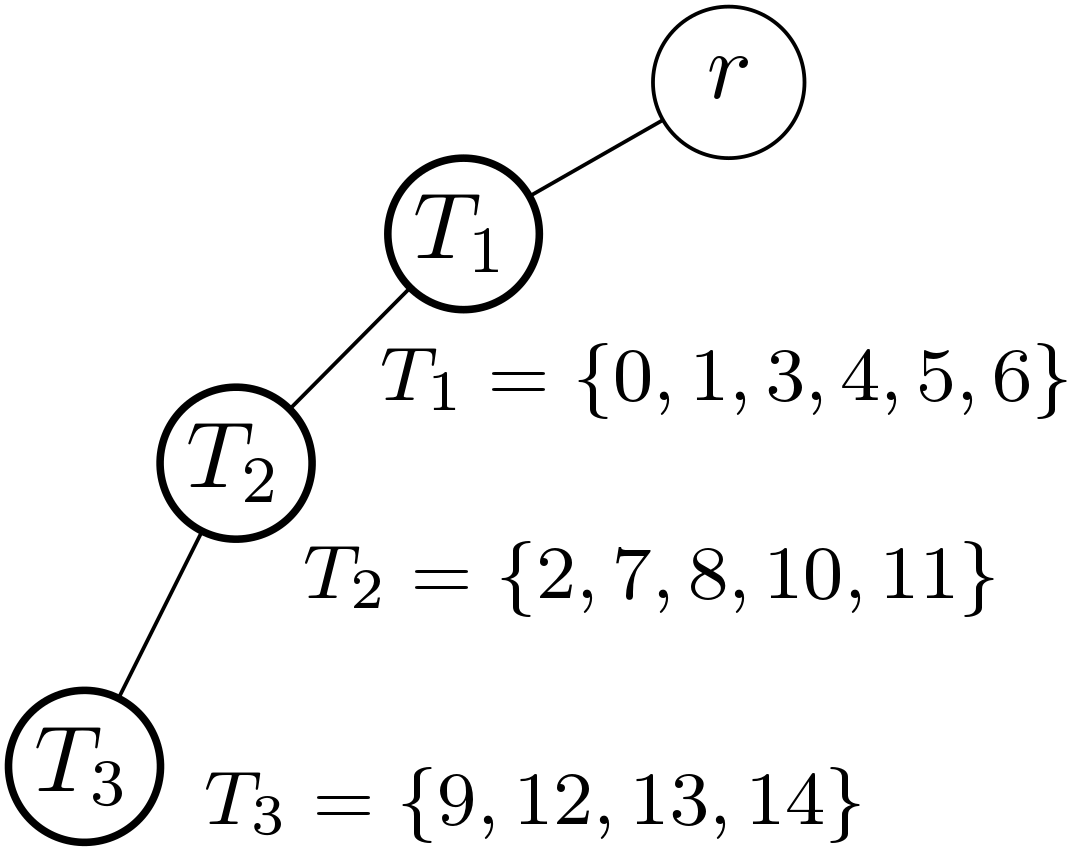
\includegraphics[width=0.7\textwidth]{exhaustive_ex1}

    \end{subfigure}\hfill%
    \begin{subfigure}{.5\textwidth}
      \centering
      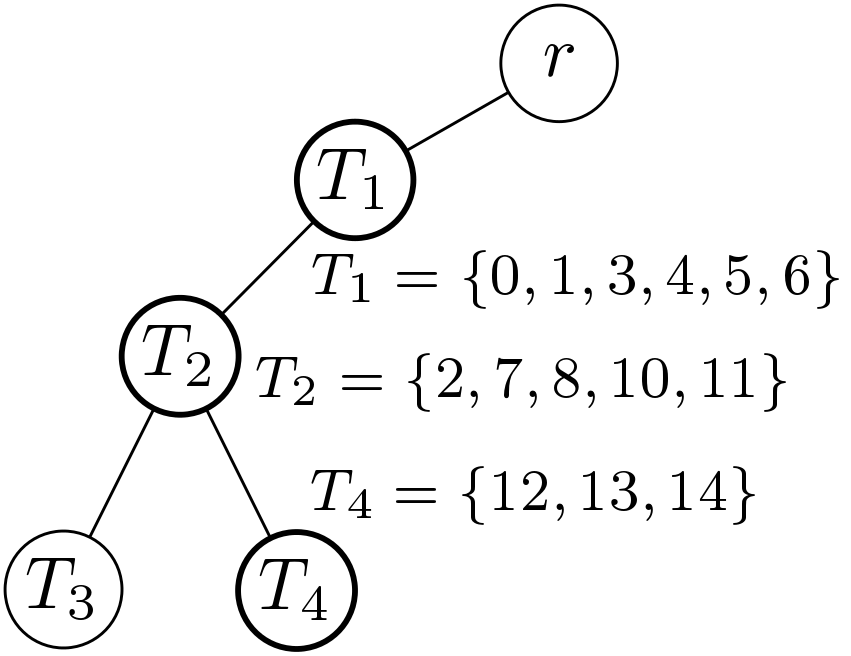
\includegraphics[width=0.7\textwidth]{exhaustive_ex1b}

    \end{subfigure}\hfill%
    \caption{En la figura de la izquierda: una descomposición de algún dibujo de $K_6$ por tres thrackles
    $T_1,T_2$ y $T_3$. Cuando $T_1$ es analizado en el algoritmo, las aristas con etiquetas $0,1,3,4,5$ y
    $6$ son agregadas al vector $coveredEdges$ y después se hace la llamada recursiva con
    $current\_thrackle=T_1$ y $LevelAt=1$, en esta llamada recursiva el algoritmo \texttt{next}
    encuentra a $T_2$ y lo agrega como parte de la colección al hacer la unión de sus aristas con el vector
    $coveredEdges$. Después se  hace la llamada recursiva con $current\_thrackle=T_2$ y $LevelAt=2$, en
    esta llamada recursiva el algoritmo \texttt{next} encuentra a $T_3$ y lo agrega como parte de la
    colección al hacer la unión  de sus aristas con el vector $coveredEdges$. Después se hace la llamada
    recursiva y se detecta que todas las aristas han sido cubiertas por lo que se actualiza el valor de
    $minAt$ y se termina la última llamada recursiva. En la figura de la derecha: Después de terminar la
    llamada recursiva se descarta $T_3$ y \texttt{next} busca, a partir de $T_2$ el siguiente thrackle
    compatible. En este ejemplo, se encuentra a $T_4$ que es un thrackle con 3 aristas. En la colección de
    los tres thrackles $T_1,T_2,T_4$ falta la arista con etiqueta 9. El algoritmo intentaría buscar el
    próximo thrackle, de tamaño 1, que cubra esta arista en la siguiente llamada recursiva. Sin embargo,
    antes de buscar un thrackle comparará las variables $LevelAt$ y $minAt$. Como son iguales, evitará
    seguir buscando un thrackle y finalizará la llamada recursiva descartando así a $T_4$. Nótese que en este momento la instancia del vector $local\_desc$ tiene los siguientes elementos: $local\_desc=\{T_3,T_4\}$. }
    \label{fig:exhaustive1}
  \end{figure}

  Una vez que se ha inicializado la matriz de disyunción podemos hacer la primer llamada recursiva a la función \texttt{exhaustive\_at} usando como parámetros un vector de enteros vacío y $LevelAt=0$.
  \begin{algorithm}
    \LinesNumbered
    % This is to hide end and get the last vertical line straight
    \SetKwBlock{Begin}{Begin}{}
    \SetAlgoLined
    \DontPrintSemicolon
    \SetKwInOut{Input}{Entrada}
    \SetKwInOut{Output}{Salida}
    \underline{función} next\_at $ (current\_thrackle,descendants,currentAt,found\_thrackle) $\;
    \Input{El thrackle actual $current\_thrackle$ desde donde se quiere encontrar otro thrackle compatible,
    un vector de vectores de enteros que representa a los descendientes de $current\_thrackle$, llamado
    $descendants$, el mejor tamaño actual de una descomposición de la gráfica completa actual $currentAt$ y
    un vector vacío $found\_thrackle$ para almacenar el resultado. .}
    \Output{ $false$ si no se encontró un thrackle compatible; $true$ si se encontró un thrackle
    compatible. El resultado es almacenado en $found\_thrackle$.}
    Sea $missing = \{0,1,2,\dots,\binom{n}{2}-1\} - coveredEdges$. \;
    $ q\gets |missing|$\;
    \If{$ q > n $ and $currentAt == 0$ }{ $q \gets n$\;}
    \If{$ q > n $ and $currentAt > 0$ }{ $q \gets n-1$\;}
    Sea $s$ el tamaño del descendiente más pequeño $i$. \;
    \If{ $s < q $ and $s > 0$ }{$q \gets s$\;}
    \If{ $descendants \neq \emptyset$ }{
      $starting\_thrackle \gets [descendants[i][0],descendants[i][1],\dots,descendants[i][q-1]]$
    }
    \ElseIf{$current\_thrackle$ es máximo o es vacío}{
      $starting\_thrackle \gets [missing[0],missing[1],\dots,missing[q-1]]$
    }
    \ElseIf{$current\_thrackle$ no es máximo ni vacío y no hay descendientes}{
      $starting\_thrackle \gets current\_thrackle$
      $q \gets |current\_thrackle|$
    }
    $p \gets 1$\;
    $ce \gets |coveredEdges|$\;
    \While{ $qp + ce < cols $ }{$p\gets p+1$}
    \If{ $currentAt + p \geq minAt$ }{
      \textbf{return} $false$
    }
    \caption{Algoritmo para encontrar el siguiente thrackle compatible.}
    \label{algo:next}

  \end{algorithm}
  \begin{algorithm}
    \LinesNumbered
    \setcounter{AlgoLine}{31}
    \SetKwBlock{Begin}{}{end}
    \Begin{
    Sea $local$ un vector de enteros vacío.\;
    \While{$true$}{
      $val \gets $\texttt{find\_next\_thrackle}($starting\_thrackle,local$)\;
      \While{ $!val$ }{
        $q \gets q-1$\;
        \If{$q == 0$ }{ \textbf{return} $false$ }
        $p \gets 1$\;
        $ce \gets |coveredEdges|$\;
        \While{ $qp + ce < cols $ }{$p\gets p+1$}
        \If{ $currentAt + p \geq minAt$ }{
          \textbf{return} $false$\;
        }
        $starting\_thrackle \gets [missing[0],missing[1],\dots,missing[q-1]]$\;
      }
      \If{  $coveredEdges \cap local == \emptyset $ }{
        \If{ $local \not\subset descendants$ }{
          $found\_thrackle \gets local$\;
          \textbf{return} $true$\;
        }
      }
    }
    }
  \end{algorithm}

  Ahora hablaremos acerca de la función \texttt{next} presentamos el pseudocódigo en el algoritmo~\ref{algo:next}. Esta función encuentra, dado un thrackle $T$ de tamaño $k$, otro thrackle compatible con $T$. Antes de empezar la búsqueda establece el tamaño $q$ del thrackle a encontrar. Esto lo hace analizando el tamaño de los descendientes de $T$, el algoritmo toma el tamaño más pequeño de estos descendientes ya que por la naturaleza del algoritmo no tiene sentido buscar un thrackle más grande que el descendiente más pequeño. Una vez que se conoce el valor de $q$ hay que elegir cuáles son las aristas en las que se iniciará la búsqueda del siguiente thrackle. Después se inicia una búsqueda secuencial y exhaustiva de un thrackle de tamaño $q$ usando la misma técnica descrita en la sección~\ref{seccion_algoritmo_kthrackles} para encontrar un thrackle de un tamaño dado. La diferencia principal es la inicialización del vector $C$ que en este caso no tendrá valores nulos sino los de las $q$ etiquetas elegidas anteriormente.

  Cuando la función \texttt{next} encuentra un thrackle $M$ con $q$ aristas se procede a verificar
  que la intersección del vector $coveredEdges$ y las etiquetas de $M$ sea vacía. Esto es para asegurar que
  $M$ sea disjunto con los otros thrackles de la colección.

  Si la función \texttt{next} no encuentra un thrackle con $q$ aristas, se repite la búsqueda de un
  thrackle con $q-1$ aristas. El tamaño mínimo de un thrackle es 1.

  Si no se logra encontrar ningún thrackle compatible se retorna el valor de $false$. Si el
  thrackle encontrado es disjunto de los thrackles que ya están en la colección se retorna el valor
  de $true$.

  Las primeras 30 líneas del pseudocódigo ilustran cómo se elige el tamaño del nuevo thrackle e inicializan el thrackle por donde se empezará la búsqueda. Las siguientes líneas describen el proceso de búsqueda de un thrackle compatible. La línea 35 llama al algoritmo de búsqueda que, como ya mencionamos, trabaja de la misma manera que el algoritmo para búsqueda de thrackles de tamaño $k$ con la diferencia de que el vector inicial no está vacío sino que tiene los contenidos de $starting\_thrackle$.

  El ciclo \texttt{while} de las líneas 34 a la 50 termina cuando sucede una de las tres situaciones siguientes
  \begin{itemize}
    \item El tamaño del thrackle compatible es 0. Esto indica que ya se ha intentado buscar thrackles compatibles con diferentes tamaños pero no se ha encontrado ninguno. Cada vez que el algoritmo no encuentra un thrackle compatible, se reduce el tamaño del thrackle a buscar en la línea 37.
    \item La comparación de la línea 44 es positiva. El segmento de código compuesto por las líneas 40 a la 45 hacen un cálculo para saber si vale la pena o no buscar un thrackle de tamaño $q$. Si se supone que en el mejor caso se necesitan $p$ thrackles de tamaño $q$ para cubrir a $K_n$ entonces el tamaño final de la descomposición en ese caso en particular es $currentAt + p$. Si esto es mayor al tamaño más pequeño encontrado para una descomposición hasta el momento ($minAt$), entonces no vale la pena seguir por ese camino y se descarta esa búsqueda.
    \item Se ha encontrado un thrackle compatible, esto es que la intersección del thrackle encontrado y las aristas cubiertas hasta el momento es vacía y que además, el thrackle encontrado no es ninguno de los descendientes de $current\_thrackle$. Esta verificación se hace en el \texttt{if} de las línea 47 a la 50.
  \end{itemize}

  En el peor caso, cada thrackle en un nodo del árbol es compatible con sus posibles hijos y por lo
  tanto, este algoritmo construiría el árbol completo. Para establecer el costo computacional del peor
  es necesario contar cuántos thrackles de tamaño $t$ existen para cada $t \in [1,10]$. Suponer que
  cada thrackle de tamaño $t$ es compatible con cada thrackle de tamaño $t-1$,$t,2$, etcétera y luego
  repetir para cada $t$ en el rango antes mencionado nos da una idea del inmenso número posible de
  nodos del árbol. Por esta razón evitamos hacer un análisis del peor caso para este algoritmo.

  Mostramos el tiempo que le tomó terminar al algoritmo, para un dibujo de ocho, siete y nueve puntos
  en la tabla~\ref{tabla_tiempo_exhaustive_at}. El tiempo de ejecución es aceptable para todo el
  trabajo exhaustivo que debe realizar el algoritmo, de aquí observamos que el peor caso no se da ya
  que hay intersección entre thrackles, sobre todo cuando los thrackles son máximos o casi máximos.
  Además, el algoritmo evita bajar en la recursión cuando el tamaño de la descomposición que va a
  analizar excede el tamaño mínimo encontrado hasta el momento.

  \begin{table}
    \centering
    \begin{tabular}{|c|c|c|}
      \hline
      $n$ & Tipo de orden & Tiempo real      \\ \hline
      $8$ & 1943          & 2 días           \\ \hline
      $7$ & 80            & 1 minuto         \\ \hline
      $6$ & 9             & 0.33 segundos    \\ \hline
    \end{tabular}
    \caption{Mostramos el tiempo de terminación para una ejecución de este algoritmo usando los tipos de orden descritos en la tabla. Estos tiempos de terminación son aceptables para esta implementación.}
    \label{tabla_tiempo_exhaustive_at}
  \end{table}


  % \subsubsection{Análisis de complejidad}
  %
  % Analizamos primero el costo de la función \texttt{exhaustive\_at} descrita en el
  % algoritmo~\ref{algo_exhaustive_at}. Las primeras 7 líneas tienen costo $O(1)$. Llamemos
  % $O(\mathcal{XT})$ al costo de la línea 12, esto es el costo de la función \texttt{next}. El costo de
  % agregar un elemento a un vector al final de este es constante por lo que la línea 15 tiene costo $O(1)$. Las operaciones de unión e intersección de conjuntos tienen costo lineal en el tamaño de los vectores de entrada, como el tamaño máximo del vector $coveredEdges$ es $\binom{n}{2}$, las operaciones de las líneas 16 y 18 tienen costo $O(n^2)$. El costo total del algoritmo depende del número de veces que se llame recursivamente a la función \texttt{exhaustive\_at}. En el peor caso, en la primera llamada a la función tratamos de cubrir una gráfica con $\binom{n}{2}$ aristas y solo podemos cubrir una, es decir, encontramos un thrackle de tamaño uno, luego la llamada recursiva será para resolver un problema de $\binom{n}{2}-1$ aristas y de nuevo, encontramos un thrackle de tamaño uno y así sucesivamente. Esto nos permite escribir una relación de recurrencia para la complejidad de este algoritmo. Sea $T(k)$ la complejidad, en el peor caso, del algoritmo \texttt{exhaustive\_at} y $k=\binom{n}{2}$: \[ T(k) = T(k-1) + O(1) + O(k^2 \frac{n-1}{2}^2) + O(\mathcal{XT}) \]
  %
  % Podemos observar que como $k=\binom{n}{2}$ entonces $n = k\frac{n-1}{2}$. Esta relación de recurrencia converge a \[ O(k^3 n^2 + \mathcal{XT}\cdot k) = O\left(\binom{n}{2}^3 n^2 + \binom{n}{2}\mathcal{XT}\right) = O(n^8 + n^2\mathcal{XT})\]
  %
  % Ahora analizamos el costo de la función \texttt{next}. Hacemos esto contando cuántas veces se
  % llamará a \texttt{next} desde un mismo nodo, para esto suponemos que el anti-thickness de la gráfica
  % completa inducida por el dibujo es mayor que el nivel donde se encuentra el nodo. Dado un thrackle
  % con $m$ aristas donde $m < n$, debemos calcular cuántos thrackles son compatibles con él. Digamos
  % que solo se han cubierto $m$ aristas, esto implica que quedan $\binom{n}{2} - m$ aristas por cubrir.
  % En el peor caso hay $\binom{\binom{n}{2}-m}{m}$ thrackles de tamaño $m$ compatibles,
  % $\binom{\binom{n}{2}-m}{m-1}$ thrackles de tamaño $m-1$ compatibles, $\binom{\binom{n}{2}-m}{m-2}$
  % thrackles de tamaño $m-2$ compatibles y de esta misma manera hasta $\binom{\binom{n}{2}-m}{1}$
  % thrackles de tamaño $1$ compatibles. Y cada uno será encontrado, no necesariamente de manera
  % subsecuente, por la función \texttt{next} desde el mismo nodo. En total hay, en el peor caso \[
  % \sum_{i=1}^m \binom{\binom{n}{2}-m}{i} \] thrackles compatibles. Como esa suma maximiza su valor
  % cuando $i=m$, podemos acotarla por $O(n^{2m})$. Luego, el valor más grande que
  % puede tener $m$ es $n-1$ podemos acotar el costo de esta función por $O(n^{2(n-1)}) = O(n^{2n})$.
  %
  % Finalmente el costo del algoritmo \texttt{exhaustive\_at} es
  % \[O(n^8 + n^2 n^{2n}) = O(n^8 + n^{2+2n}) = O (n^{2+2n}).\]



\subsection{Algoritmo para dar el número de cruce de un thrackle máximo}
  \label{secc:algo_cnthracklemax}

  Este algoritmo fue diseñado para resolver el siguiente problema:
  \begin{itemize}
    \item[] Problema: Dado un thrackle geométrico calcular su número de cruce.
    \item[] Entrada: Las aristas del thrackle representadas en un arreglo booleano.
    \item[] Salida: El número de cruce del thrackle.
  \end{itemize}

  Calculamos el número de cruce de un thrackle como describimos en la
  sección~\ref{secc:cnthracklemax}. Recordemos que para un thrackle con $m$ aristas el número de cruce
  es \[ \binom{m}{2} - \sum_{u\in V(T)} \binom{deg(u)}{2}. \]

  Mostramos el pseudocódigo del algoritmo para realizar los cálculos en el algoritmo~\ref{algo_cnthracklemax}.

  \begin{algorithm}[b]
    \DontPrintSemicolon
    \SetKwInOut{Input}{Entrada}
    \SetKwInOut{Output}{Salida}
    \underline{función CrossingNumberThrackle} $(E,n)$\;
     \Input{Un arreglo booleano E, de tamaño $\binom{n}{2}$, que representa a las aristas del thrackle.}
     \Output{Un entero $r$ igual al número de cruce del thrackle inducido por $E$.}
     $i,j,c \gets 0$\;
     Sea $degs[n]$ un arreglo de enteros, de tamaño $n$\;
     $th\_size \gets 0$\;
     $sum \gets 0$\;
     $r \gets 0$\;
     \For{$i=0,\dots,\binom{n}{2}$}{
      \If{$E[i] == 1$}{
        $th\_size \gets th\_size + 1$\;
      }
     }
     \For{$i = 0,\dots, n$}{
         \For{$ j = i+1, \dots, n$}{
             \If{$E[c]$}{
                 $degs[i] \gets degs[i]+1$\;
                 $degs[j] \gets degs[j]+1$\;
             }
             $c \gets c+1$\;
         }
     }
     $ans \gets th\_size\cdot \frac{(th\_size-1)}{2}$\;
     $sum \gets 0$\;
     \For{$i = 0,\dots, n$}{
         $sum \gets sum + degs[i]\cdot\frac{(degs[i]-1)}{2}$\;
     }
     $r \gets ans-sum$\;
     \textbf{return} $r$\;
    \caption{Algoritmo para calcular el número de cruce de un thrackle geométrico.}
    \label{algo_cnthracklemax}
  \end{algorithm}

  \subsubsection{Análisis de complejidad}

  Este algoritmo es secuencial. El ciclo de la línea 7, recorre un arreglo de tamaño
  $\binom{n}{2}$ lo que aporta $O(n^2)$ a la complejidad. Los ciclos anidados de las
  líneas 10 y 11 realizan $n + n-1 + n-2 + \dots + 1$ operaciones con complejidad $O(1)$,
  lo que aporta $O(n^2)$  a la complejidad del algoritmo. Finalmente, el ciclo de la
  línea 18 recorre un arreglo de tamaño $n$, lo que aporta $O(n)$ a la complejidad.

  Así, la complejidad total del algoritmo es \[ O(n^2) + O(n^2) + O(n) = O(n^2)\].
